\documentclass[12pt, twoside, openany]{report}

%%%%%%%%%%%%%%% moje dodanie

\usepackage[T1]{fontenc}
\usepackage[polish]{babel}
\usepackage[utf8]{inputenc}
\usepackage{lmodern}
\selectlanguage{polish}
\usepackage{latexsym}
\usepackage{cite}
\usepackage{verbatim}
\usepackage{listings}
\usepackage{float}
\usepackage{lipsum} % for dummy text
\usepackage{placeins}
\usepackage[xindy]{glossaries}
\usepackage{mfirstuc}
\usepackage{listings}



\lstset{
  basicstyle=\ttfamily\small,
  columns=fullflexible,
  showstringspaces=false,
  commentstyle=\color{gray}\upshape
}
\lstdefinelanguage{XML}
{
  basicstyle=\ttfamily\tiny,
  morestring=[b]",
  morestring=[s]{>}{<},
  morecomment=[s]{<?}{?>},
  stringstyle=\color{black},
  identifierstyle=\color{blue},
  keywordstyle=\color{cyan},
  morekeywords={xmlns,version,type}% list your attributes here
}
\lstdefinestyle{sharpc}{language=[Sharp]C, frame=lr, rulecolor=\color{blue!80!black}}



%%%%%%%%%%%%%%%%%%%%%%%%%%%

\usepackage[dvips]{graphicx,color,rotating}
%\usepackage[cp1250]{inputenc}
\usepackage{t1enc}
\usepackage{a4wide}
\usepackage{amsfonts}
\usepackage{amsmath}
\usepackage{enumerate}
\usepackage{verbatim}
\usepackage[MeX]{polski}
\usepackage[T1]{fontenc}
\usepackage{geometry}
\geometry{left=25mm,right=25mm,%
bindingoffset=10mm, top=25mm, bottom=25mm}
%\usepackage{amssymb, latexsym}
\usepackage{amsthm}
\usepackage{palatino}
\usepackage{array}
\usepackage{pstricks}
\usepackage{textcomp}
\theoremstyle{definition}
\newtheorem{theorem}{Twierdzenie}[section]
\newtheorem{remark}{Uwaga}[section]
\newtheorem{definition}{Definicja}[section]
\newtheorem{alg}{Algorytm}[chapter]
\newtheorem{prz}{Przypadek}[section]
\newtheorem{np}{Przykład}[section]
\newtheorem{lemma}[theorem]{Lemat}
\linespread{1.5}
\newcommand*{\norm}[1]{\left\Vert{#1}\right\Vert}
\newcommand*{\abs}[1]{\left\vert{#1}\right\vert}
\newcommand*{\om}{\omega}

\author{Paweł Kupidura, Hubert Rosiak, Kacper Trojanowski}
\title{Efektywna implementacja wybranego algorytmu optymalizacji globalnej}

\makeglossaries

\begin{document}
\begin{titlepage}
\pagestyle{empty}

\noindent
\begin{Large}
\begin{table}[t]
\centering
\begin{tabular}[t]{lcr}
 
\includegraphics[width=70pt,height=70pt]{PW} & POLITECHNIKA WARSZAWSKA & 
\includegraphics[width=70pt,height=70pt]{MiNI}\\
& WYDZIAŁ MATEMATYKI & \\
& I NAUK INFORMACYJNYCH &
\end{tabular}
\end{table}

% \vfill
\begin{center}PRACA DYPLOMOWA INŻYNIERSKA\end{center}
\begin{center}INFORMATYKA\end{center}\end{Large}
% \vfill
\begin{center}
\Huge
\textbf{Efektywna implementacja wybranego algorytmu optymalizacji globalnej}
\end{center}
% \vfill\vfill
\vfill
\begin{center}
\Large
Autorzy:\\
\LARGE
Paweł Kupidura\\
Hubert Rosiak\\
Kacper Trojanowski
\end{center}
\vfill
\begin{center}
\Large
Promotor: mgr inż. Michał Okulewicz
\end{center}
\vfill
\begin{center}
\large
Warszawa, wrzesień 2016
\end{center}
\newpage
\hfill
\begin{table}[b]
\centering
\begin{tabular}[t]{ccc}
............................................. & \hspace*{100pt} & .............................................\\
podpis promotora & \hspace*{100pt} & podpis autora
\end{tabular}
\end{table}


% \maketitle
\end{titlepage}

\thispagestyle{empty}
\newpage
\pagestyle{headings}
\setcounter{page}{1}
\hyphenation{Syl-ves-tra}
\hyphenation{Syl-ves-ter-a}

\begin{abstract}
W niniejszej pracy inżynierskiej prezentujemy rozproszony system do optymalizacji umożliwiający uruchomienie obliczeń na klastrze złożonym z kilku komputerów, którego bazowym silnikiem optymalizacyjnym jest algorytm Particle Swarm Optimization. Program napisany został ze szczególnym uwzględnieniem optymalizacji funkcji ciągłych z benchmarku BBOB jednak umożliwia programiście rozszerzenie funkcjonalności do dowolnego rodzaju funkcji. Algorytm zaimplementowany został w postaci biblioteki w technologii .NET umożliwiającej dopasowanie się do sprzętu, na którym jest uruchamiana wykorzystując wieloprocesorowość lokalnej maszyny oraz umożliwiającej uruchomienie obliczeń rozproszonych na wielu komputerach jednocześnie wykorzystując usługi WCF. Biblioteka pozwala też na wykorzystanie do obliczeń równoległych procesorów graficznych obsługujących technologię CUDA. Jako test działania prezentujemy wyniki testów naszej biblioteki na benchmarku optymalizacyjnym BBOB.

%W niniejszej pracy inżynierskiej prezentujemy stworzoną przez nas implementację algorytmu Particle Swarm Optimization. Algorytm zaimplementowany został w postaci biblioteki w technologii .NET umożliwiającej dopasowanie się do sprzętu, na którym jest uruchamiana wykorzystując wieloprocesorowość lokalnej maszyny oraz umożliwiającej uruchomienie obliczeń rozproszonych na wielu komputerach jednocześnie wykorzystując usługi WCF. Biblioteka pozwala też na wykorzystanie do obliczeń równoległych procesorów graficznych obsługujących technologię CUDA. Prezentujemy również wyniki testów naszej biblioteki m.in. na benchmarku optymalizacyjnym BBOB.
\end{abstract}

\tableofcontents

%-----------Początek części zasadniczej-----------

\chapter{Słowniczek}

\textbf{Algorytm optymalizacyjny} - Algorytm rozwiązujący problem optymalizacji.\\
\textbf{Benchmark} - Sposób oceny jakości sprzętu lub programu komputerowego polegający na uruchomieniu zestawu testów i porównaniu ich ze znanymi standardami.\\
\textbf{Black-box optimization} - Rodzaj zadania optymalizacyjnego, w którym algorytm optymalizacyjny nie zna postaci funkcji celu, a może jedynie zapytać się o jej wartość w danym punkcie.\\
\textbf{CUDA} - Platforma programistyczna firmy NVIDIA umożliwiająca wykorzystywanie procesorów graficznych w obliczeniach\\
\textbf{Framework} - Platforma programistyczna. Szkielet aplikacji definiujący jej ogólną strukturę i mechanizm działania lub dostarczający komponenty wykonujące określone zadania.\\
\textbf{Funkcja celu} - Funkcja, której ekstremum jest poszukiwane w zagadnieniu optymalizacji.\\
\textbf{GPU} - Graphics Processing Unit. Wyspecjalizowana jednostka obliczeniowa typu SIMD przystosowana do efektywnego przetwarzania grafiki komputerowej. Może być również wykorzystywana do obliczeń równoległych na dużych zbiorach danych.\\
\textbf{Klaster obliczeniowy} - Zespół węzłów obliczeniowych połączonych ze sobą siecią, umożliwiający prowadzenie wspólnych obliczeń.\\
\textbf{Marshalling} - Zmiana sposobu reprezentacji danych w pamięci do formatu właściwego dla transmisji do innego fragmentu programu.
\textbf{Metaheurystyka} - Ogólny algorytm do rozwiązywania problemów obliczeniowych, który można dostosować do konkretnego problemu.\\
\textbf{Obliczenia rozproszone} - Obliczenia prowadzone jednocześnie na wielu jednostkach obliczeniowych, mogących różnić się między sobą architekturą i położeniem geograficznym, ale komunikujących się ze sobą i mogących korzystać ze wspólnych zasobów. Synchronizacja między jednostkami zachodzi w szerszej skali niż w przypadku obliczeń równoległych.\\
\textbf{Obliczenia równoległe} - Zsynchronizowane obliczenia prowadzone jednocześnie na kilku jednostkach obliczeniowych, zazwyczaj procesorach na jednej maszynie.\\
\textbf{Optymalizacja} - Zagadnienie znajdowania wartości ekstremalnej (najczęściej minimalnej lub maksymalnej) zadanej funkcji celu.\\
\textbf{PSO} - Particle Swarm Optimization. Ewolucyjny algorytm optymalizacyjny, wykorzystujący populację cząstek poruszających się w przestrzeni możliwych rozwiązań.\\
\textbf{SIMD} - Single instruction, multiple data. Jeden z rodzajów architektur jednostek obliczeniowych, w którym wiele strumieni danych przetwarzanych jest w oparciu o pojedynczy strumień rozkazów.\\
\textbf{WCF} - Windows Communication Foundation. Platforma programistyczna wykorzystywana przy budowie aplikacji korzystających z komunikacji sieciowej.\\
\textbf{Wrapper} - Zestaw funkcji i klas mających za zadanie pośredniczenie między dwiema różnymi warstwami aplikacji.\\



%%%%%%%%%%%%%%%%%%%%%%%%%%%%%%%%%%%%%%%%%%%%%%%%%%%%%%%%%%%%%%%%%%%%%

\chapter{Wstęp teoretyczny} %[bez wspominania naszej pracy]

\section{Czym jest PSO?} %nieformalnie

PSO (Particle Swarm Optimization) jest metodą rozwiązywania problemów optymalizacyjnych należącą do klasy metaheurystycznych algorytmów ewolucyjnych, wzorowaną na spotykanym w przyrodzie zachowaniu się rojów i stad zwierząt. Po raz pierwszy przedstawiona została w pracy Eberhardta  i Kennedy’ego w 1995 r. \cite{Pso}. W ogólności polega ona na potraktowaniu potencjalnych rozwiązań zagadnienia optymalizacyjnego jako ,,cząstek'', które poruszają się w przestrzeni możliwych rozwiązań. Ruch cząsteczek odbywa się w czasie dyskretnym - w każdej iteracji głównej pętli algorytmu każda z cząstek przemieszcza się o wektor prędkości, który zależy od prędkości w poprzedniej iteracji, najlepszego dotychczas znalezionego przez sąsiadów rozwiązania (globalnego), najlepszego rozwiązania znalezionego przez daną cząstkę (lokalnego) oraz od czynnika losowego. Na poziomie praktycznym za przestrzeń rozwiązań najczęściej wybiera się n-wymiarową przestrzeń Euklidesową, zaś zagadnieniem optymalizacyjnym jest znalezienie minimum (maksimum) pewnej funkcji rzeczywistej określonej na pewnym podzbiorze tej przestrzeni. Ze względu na fakt, iż PSO jest jedynie (meta)heurystyką, szczegóły algorytmu i jego parametry można dobierać odpowiednio do konkretnego zastosowania.


\section{Definicja algorytmu} %formalnie

%zrobić tu albo wcześniej słownik PSO – co to jest (formalnie) rój, sąsiedztwo itp.
 
Klasyczna wersja algorytmu (wg. \cite{Pso}), zakładająca pełne sąsiedztwo cząstek [pełny graf sąsiedztwa] wygląda następująco:

\begin{enumerate}
\item Inicjalizacja cząstek:

\begin{enumerate}
\item Utwórz cząstki rozmieszczone losowo (według rozkładu jednostajnego) w całej przestrzeni rozwiązań;
\item Jako najlepszą znaną pozycję ustaw dla każdej z cząstek jej pozycję startową; 
\item Zaktualizuj optimum globalne znajdując pozycję cząstki o najmniejszej wartości funkcji celu; 
\item Nadaj cząstkom losowe prędkości z pewnego zakresu (według rozkładu jednostajnego; 
\end{enumerate}

\item Główna pętla algorytmu - dopóki nie został spełniony warunek stopu (określona liczba iteracji lub znalezienie wartości odpowiednio bliskiej znanemu optimum globalnemu), wykonuj:
\begin{enumerate}

\item Dla każdej z cząstek oblicz jej nową prędkość w następujący sposób:

\begin{center}

$v_{t+1} \leftarrow \omega \cdot v_t + \phi_1 \cdot r_1 \cdot p + \phi_2 \cdot r_2 \cdot g$

\end{center}

gdzie:
$v_{t+1}$ - wektor prędkości w iteracji $t+1$,\\
$v_t$ - wektor prędkości w iteracji $t$,\\
$p$ - wektor łączący obecne położenie cząstki z jej najlepszą znaną pozycją,\\
$g$ - wektor łączący obecne położenie cząstki z najlepszą globalnie pozycją,\\
$\omega$ - współczynnik bezwładności,\\
$\phi_1, \phi_2$ - ustalone przez użytkownika parametry (wagi),\\
$r_1, r_2$ - liczby z przedziału $[0,1]$ losowane w każdej iteracji\\

\item Przesuń każdą cząstkę o jej nowy wektor prędkości;
\item Dla każdej z cząstek oblicz funkcję celu w nowym położeniu i, jeżeli to możliwe, zaktualizuj najlepszą dotychczasową pozycję cząstki; 
\item Zaktualizuj optimum globalne; 
\end{enumerate}
\end{enumerate}

\begin{figure}[H]
    \centering
 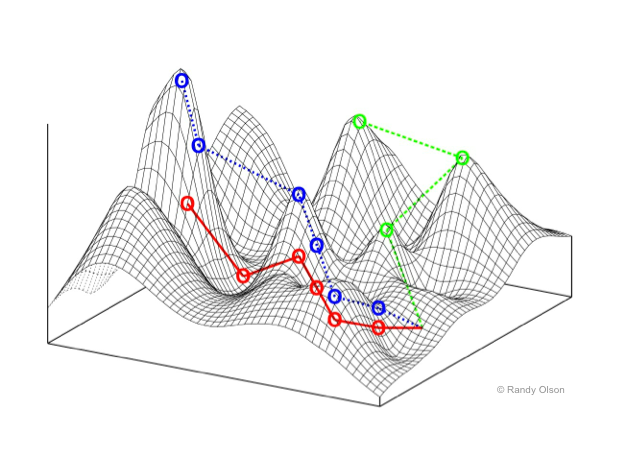
\includegraphics[width=1\textwidth,natwidth=610,natheight=642]{PSO_2D.png}
 \caption{Algorytm PSO w dwóch wymiarach \cite{PSO_2D_img}}
\end{figure}

\section{Dotychczasowy stan badań nad PSO}

Od momentu powstania w 1995 r. algorytm ten zyskał popularność i szerokie zastosowanie. Był też tematem licznych prac naukowych i opracowań, mających na celu próbę jego lepszego zrozumienia i poprawy skuteczności oraz zbadanie zachowania dla wielu różnych klas problemów optymalizacyjnych.
%[do słownika problem optymalizacyjny]. 

Elastyczność definicji algorytmu sprawia, że wiele jego parametrów 
%[i procedur] 
można zmieniać i dostosowywać do aktualnych potrzeb. Skuteczność standardowej wersji PSO 
%[do słownika SPSO]
w zależności od parametrów takich, jak: wielkość roju cząstek, sposób inicjalizacji położeń i prędkości oraz ich aktualizacji w głównej pętli algorytmu czy topologia sąsiedztwa cząstek roju została zbadana w pracy \cite{SPso} 
%[może to rozbić na parametry, a dalej o procedurach?]

%[Za \cite{ComprLearnPso}]
Dobre podsumowanie stanu badań nad PSO znajduje się w pracy \cite{ComprLearnPso}, której autorzy wspominają, iż szybko zauważono, że niektóre słabości standardowej, opisanej powyżej wersji algorytmu, można usprawnić, wprowadzając do niego pewne dodatkowe elementy, często inspirowane lub wprost pochodzące od innych algorytmów optymalizacyjnych. Powstały w ten sposób różne warianty i hybrydy algorytmu PSO.

Jedna z prostszych modyfikacji 
%[źródło?] 
wprowadza parametr ,,bezwładności $\omega$'' do wzoru wyliczającego zaktualizowaną prędkość każdej cząstki w następujący sposób:

Kontrolowanie bezwładności ma umożliwiać zrównoważenie zdolności eksploatacyjnych i eksploracyjnych algorytmu 
%[do słownika]
 – duża wartości sprzyja eksplorowaniu większego obszaru, zaś mniejsza – skupienie się na bardziej lokalnym przeszukiwaniu. Bezwładność może też być dynamicznie zmieniana w trakcie wykonywania algorytmu – jej liniowe zmniejszanie się względem liczby iteracji przedyskutowano w \cite{ModPsoInertia}, zaś właściwy dobór parametrów algorytmu omówiono w \cite{ParamSelPso}. Inne, nieliniowe metody zmiany bezwładności opisano w \cite{PsoFuzzyInertia}. W pracy \cite{SelfOrgHPso} dla odmiany, parametr w ustawiany jest na 0 za wyjątkiem sytuacji reinicjalizacji.
%[co to?]
W trakcie działania algorytmu można dynamicznie modyfikować także inne jego parametry, jak np. prędkość maksymalną – wariant algorytmu implementujący jej liniowy spadek opisany został w \cite{VmaxPso}.

Duży wpływ na wydajność algorytmu ma też w oczywisty sposób topologia 
%[do słownika topologia roju] 
roju cząstek. J. Kennedy (jeden z twórców pierwotnej wersji algorytmu) stwierdził, że mniej liczne sąsiedztwo każde cząsteczki sprawdza się lepiej w przypadku bardziej złożonych problemów 
%[co to znaczy?]
, podczas gdy liczne sąsiedztwo działa lepiej dla prostych problemów \cite{TopologyPso}, \cite{PopStructPso}. Ciekawym rozwiązaniem jest zaproponowane w \cite{PsoNeighOp} dynamicznie dostosowywane sąsiedztwo, które stopniowo powiększa się, aż do momentu objęcia całego roju. W artykule \cite{MultiobjDynNeighPso} Hu i Eberhart zaproponowali inny sposób dynamicznego modyfikowania sąsiedztwa – w każdej iteracji algorytmu cząsteczka na nowo wybiera sobie za sąsiadów te cząstki, które są jej bliskie według pewnej metryki 
%[jakiej?]
. Wariant UPSO (Unified Particle Swarm Optimizer) \cite{UPso} stara się połączyć globalną eksplorację z lokalną eksploatacją.
%[jak? Co to znaczy?]
Wprowadzone przez Mendesa i Kennedy’ego \cite{FullyInformedPso} Fully Informed PSO różni się od klasycznej wersji tym, że w momencie aktualizacji prędkości cząstki pod uwagę bierze się nie tylko informację pochodzącą od najlepszego sąsiada, ale, z odpowiednimi wagami, również  informacje zebrane od pozostałych sąsiadów cząstki. Wagę, jaką przypisuje się informacji od każdej z cząstek sąsiedztwa zależy m.in. od jej aktualnej wartości funkcji celu oraz rozmiaru samego sąsiedztwa. 
%[co dzięki temu zyskujemy?] [Inny wariant, „Comprehensive learning PSO.]
 Z kolei fitness-distance-ratio-based PSO (FDR-PSO) \cite{FitnessDistRatio}, wprowadza pewne dodatkowe interakcje 
%[jakie?] 
między pobliskimi cząstkami podczas aktualizacji prędkości.

Innym sposobem usprawnienia działania algorytmu, który doczekał się licznych opracowań, jest hybrydyzacji PSO, czyli próba połączenia z innymi algorytmami i technikami optymalizacji. Jednym z popularnych pomysłów jest wprowadzenie do PSO operacji znanych z innych algorytmów ewolucyjnych, takich jak selekcja, krzyżowanie i mutacja, w celu zachowania cech najlepszych cząstek roju, bądź też wprowadzenie większej różnorodności do populacji, mające zapobiec zbieżności do lokalnych minimów \cite{SelectionPso},\cite{HybridPsoBreedingSubpop}. Z tego samego powodu wprowadza się różne mechanizmy unikania kolizji między \cite{CollisionAvoiding}, takie jak relokacja cząstek, które znalazły się zbyt blisko siebie \cite{PsoCriticality}. Operatory mutacji są też stosowane do mutowania 
%[?]
 parametrów algorytmu takich jak opisana wcześniej bezwładność \cite{EPso}. W pracy \cite{HybridPsoBreedingSubpop}, rój cząstek dzielony jest na mniejsze subpopulacje, zaś ,,breeding operator'' 
 %[?]
  jest stosowany w obrębie jednej z nich lub też między nimi w celu zwiększenia różnorodności roju. Odpowiedzią na problem zbyt wczesnej zbieżności cząsteczek do minimów lokalnych, które może spowodować ominięcie minimum globalnego, jest wprowadzenie negatywnej entropii \cite{DissipativePso}. W \cite{ComputGlobOptPso} z kolei, przedstawione zostały techniki, których celem jest znalezienie jak największej liczby minimów funkcji kosztu poprzez zapobieganie poruszaniu się cząsteczek w kierunku znanych już minimów.
Jednym z innych wariantów mających poprawić wyniki otrzymywane przez PSO na funkcjach multimodalnych 
%[wielomodalnych?]
 jest tzw. cooperative PSO (CPSO-H), używające jednowymiarowych rojów do oddzielnego przeszukiwania każdego wymiaru zadanego problemu, których wyniki są następnie w odpowiedni sposób łączone.

\section{Istniejące implementacje i zastosowania PSO}

%[na podstawie \cite{EObjGeneral}]

Wspomniana popularność algorytmów ewolucyjnych, a wśród nich PSO, poskutkowała ich wykorzystaniem zarówno do badań teoretycznych jak i praktycznych zastosowań. Spowodowało to powstanie wielu implementacji tych algorytmów, z których jednak każda posiada swoje wady i ograniczenia. Jednym z podstawowych problemów wielu bibliotek jest narzucona z góry, sztywna reprezentacja obiektów, które chcemy poddać procesowi ewolucji, jak i operatorów ewolucyjnych – często pozwalają one jedynie na korzystanie niewielkiego zbioru predefiniowanych reprezentacji, co zmusza do ,,spłaszczania'' bardziej skomplikowanych struktur danych do typowych postaci, na których operują istniejące biblioteki, takich jak ciągi bitów, czy tablice liczb – podejście takie może znacząco utrudnić zarówno zrozumienie, jak i rozwiązanie problemu.

Jedną z odpowiedzi na opisane wyżej problemy jest napisana w języku C++ open source’owa biblioteka EOlib (Evolving objects library), zawdzięczająca swoją elastyczność podejściu obiektowemu – każda struktura danych jak i każdy operator jest obiektem. Biblioteka zawiera kilka predefiniowanych reprezentacji, ale każdy użytkownik może stworzyć swoje własne ,,ewoluujące obiekty'', o ile tylko implementują one wymagany interfejs, tzn. zapewniają możliwość inicjalizacji, selekcji osobników oraz ich reprodukcji i mutacji (lub krzyżowania) 
%[do słownika genetycznego]
. 

Kolejną zaletą EOlib jest odejście od często stosowanego, ale ograniczającego założenia, iż funkcja celu musi być funkcją skalarną – w bibliotece tej może ona być dowolnego typu.
%[jest obiektem?]

Biblioteka Eolib jest podstawową popularnego frameworka Paradiseo (typu white-box, czyli dającego programiście wgląd w szczegóły implementacji), służącego do tworzenia metaheurystyk.
%[co to znaczy? słownik?]
Składa się on z modułów: Paradiseo-EO -  obsługującego algorytmy populacyjne, Paradiseo-MOEO – służącego do optymalizacji [wielokryteriowej], Paradiseo-MO – dla problemów z jednym rozwiązaniem, Paradiseo-PEO – narzędzia do tworzenia rozwiązań równoległych i rozproszonych.

%[może jakieś inne zastosowania lub implementacje?]

\section{Równoległe i rozproszone PSO}
%[tak ogólnie o zrównoleglaniu/rozpraszaniu obliczeń [ewolucyjnych?] - może „Obliczenia równoległe i rozproszone”]

Obliczenia rozproszone polegają na uruchomieniu jednoczesnych obliczeń na więcej niż jednym komputerze. W przypadku algorytmu PSO rozproszenie obliczeń można wykonać na wiele sposobów - na przykład za pomocą jednego wielkiego roju cząstek działającego równolegle na wszystkich maszynach lub też za pomocą większej liczby mniejszych rojów.  

%[jakie zalety mają obliczenia równoległe/rozproszone]
%...
%[jakie są trudności]
%...

%[resztę rozdziału można usunąć – wystarczy pierwszy akapit z kolejnego %działu, aby opisać równoległą naturę PSO]

Standardowa wersja algorytmu PSO wprost ze swojej natury nadaje się do zrównoleglenia obliczeń - niezależnie czy mówimy o zrównolegleniu na poziomie roju czy części roju cząstek.
Obliczanie nowej prędkości dla każdej z cząstek zależy tylko od jej własności i własności sąsiadów z poprzedniej iteracji, zatem w oczywisty sposób potrzeby synchronizacji sprowadzają się do zaktualizowania zbioru cząstek 
%[?]
 i wyboru globalnego minimum (maximum). 

\subsection{Stan badań nad równoległym i rozproszonym PSO}

%[za \cite{AccelParallelPso} oraz \cite{ComparisonParallelGpuPso}]

W niniejszym podrozdziale przedstawiamy obecny stan badań nad zrównolegleniem i rozproszeniem algorytmu PSO na podstawie dostępnej literatury.

Algorytm PSO jest algorytmem w oczywisty sposób nadającym się do zrównoleglenia obliczeń, ze względu na fakt, że poszczególne osobniki populacji (w przypadku PSO – cząstki) 
%[?]
 są od siebie w mniejszym bądź większym stopniu niezależne i przeprowadzają samodzielne obliczenia. Dodatkowo, dla trudnych problemów optymalizacyjnych o wielu wymiarach, potrzebna liczba cząstek może być bardzo znacząca, co skłania do poszukiwania poprawy wydajności i przyspieszenia obliczeń właśnie na drodze zrównoleglenia czy rozproszenia. 
Oczywiście wraz z zaletami programowania równoległego pojawiają się charakterystyczne dla niego problemy, które należy rozwiązać, takie jak: skalowalność, synchroniczna i asynchroniczna implementacja, spójność i komunikacja sieciowa. 
%[może wyjaśnić te problemy? Chyba, że będą opisane w poprzednim rozdziale]

W pracach \cite{AccelParallelPso} oraz \cite{ComparisonParallelGpuPso} przedstawiono po krótce niektóre z zaproponowanych do tej pory rozwiązań problemu paralelizacji algorytmu PSO. Większość z nich oparta jest na klastrach komputerów wymieniających się między sobą wiadomościami.
%[?]
Niektóre z implementacji używają popularnego standardu OpenMP. Warto wspomnieć, że analiza przeprowadzona w \cite{Pso8} wskazuje, że pewien rodzaj równoległego PSO, w którym cząstki aktualizuje się grupami, nie zawsze wymagać większej liczby operacji niż implementacja sekwencyjna, w której cząstki aktualizowane są jedna po drugiej, zajmując przy tym mniej czasu.

PSO jest w naturalny sposób równoległe na poziomie algorytmicznym 
%[co to jest równoległość na poziomie algorytmicznym?] [embarassingly parallel]
, jednakże zaimplementowanie tej równoległości nie jest już takie oczywiste – wśród głównych problemów, z którymi należy się zmierzyć, są komunikacja %[między węzłami obliczeniowymi? Cząstkami?]
 i równoważenie obciążenia, przy czym zagadnienia te są ze sobą powiązane. W algorytmie PSO największym kosztem obliczeniowym jest zazwyczaj ewaluacja funkcji celu dla każdej cząstki. Jeżeli ewaluacja ta jest relatywnie kosztowna, koszt komunikacji można zaniedbać i pierwszoplanowym problemem staje się równoważenie obciążenia między węzłami obliczeniowymi.
 %[?] 
W przeciwnym przypadku względnie niskiego kosztu ewaluacji funkcji celu, koszt komunikacji może dominować obliczenia.

Wśród stosowanych podejść do problemu zrównoleglenia algorytmu PSO można wyróżnić dwa główne: podejście synchroniczne i asynchroniczne. W pierwszym z nich wszystkie procesory czekają na zakończenie ewaluacji funkcji celu dla wszystkich cząsteczek przed przejściem do kolejnej iteracji. Przeprowadzono wiele eksperymentów, które sugerują, że efektywność zrównoleglenie (parallel efficiency%[do słownika? Do poprzedniego rozdziału?]
) spada wraz z liczbą procesorów i jest daleka od idealnej 100 procent.
%[źródło]
W celu zrównoważenia nieefektywności wynikającej z nierównego rozłożenia obliczeń, zaproponowano podejście asynchroniczne - pozwala ono każdemu procesorowi (procesowi, wątkowi) przejść niezależnie do kolejnej iteracji po ukończeniu obliczania funkcji celu. Wyniki eksperymentów pokazały znaczący wzrost efektywności w porównaniu z wersją synchroniczna. 
%[źródło]

Jednym ze sposobów zrównoleglenia obliczeń jest wykorzystanie w tym celu procesorów graficznych (GPU). Skupimy się tutaj głównie na procesorach graficznych wspierających architekturę CUDA (Compute Unified Device Architecture) \cite{CudaProgGuide} stworzoną przez firmę NVIDIA. Platforma ta zyskała bardzo dużą popularność jako prostsza i bardziej intuicyjna alternatywa dla np. standardu OpenCL.

%[może tutaj opisać architekturę CUDA, albo w ogóle gdzieś wcześniej, żeby było wiadomo, o czym mówimy w kolejnym akapicie]

W artykule \cite{GpuBasedPso} opisana została paralelizacja 
%[?]
 standardowego PSO (SPSO) na GPU z 11-krotnym przyspieszeniem względem CPU. Implementacja ta wykorzystuje topologię pierścienia, a więc umożliwia każdej cząstce komunikację z jedynie dwoma sąsiadami. Dzięki temu nie ma potrzeby równoległego poszukiwania najlepszego sąsiada podczas aktualizacji prędkości, co ogranicza konieczność komunikacja między wątkami. Z kolei rozwiązanie opisane w \cite{PsoCuda} bazuje na pomyśle utworzenia wątków GPU w liczbie równej liczbie cząstek roju pomnożonej przez liczbę wymiarów (co jednak niesie ze sobą konieczność ograniczenia maksymalnej liczby wymiarów rozważanego problemu optymalizacyjnego), który to w pewnych szczególnych przypadkach daje nawet 50-krotne przyspieszenie względem implementacji sekwencyjnej. Innym ciekawym rozwiązaniem jest zaproponowana w \cite{PsoGraphHardLocPat} hybrydyzacja algorytmu PSO z algorytmem ,,pattern search'', która na GPU może osiągnąć lepsze wyniki niż każdy z tych algorytmów z osobna. 
 %[Autorzy \cite{ComparGpuPso} porównujący warianty PSO na GPU jednak zrównoleglają jedynie ewaluację funkcji kosztu – daje to nawet 27-krotne przyspieszenie, jednakże autorzy \cite{ComparisonParallelGpuPso} uważają, że rozwiązanie to nie wydaje się być skalowalne dla większych rojów, jako, że inicjalizacja, poszukiwanie najlepszej cząstki oraz aktualizacja prędkości i położenia są wykonywane sekwencyjne.]
Artykuł \cite{BlockOccupancyGpu} bada zależność między wydajnością algorytmu PSO, a wielkością bloku wątków, uzyskując przy tym 43-krotny zysk.


\chapter{Zaimplementowany system optymalizacyjny}

\section{Architektura węzła obliczeniowego}

Poniżej przedstawiamy najważniejsze klasy składające się na pojedynczy węzeł obliczeniowy. 

\begin{figure}[H]
    \centering
 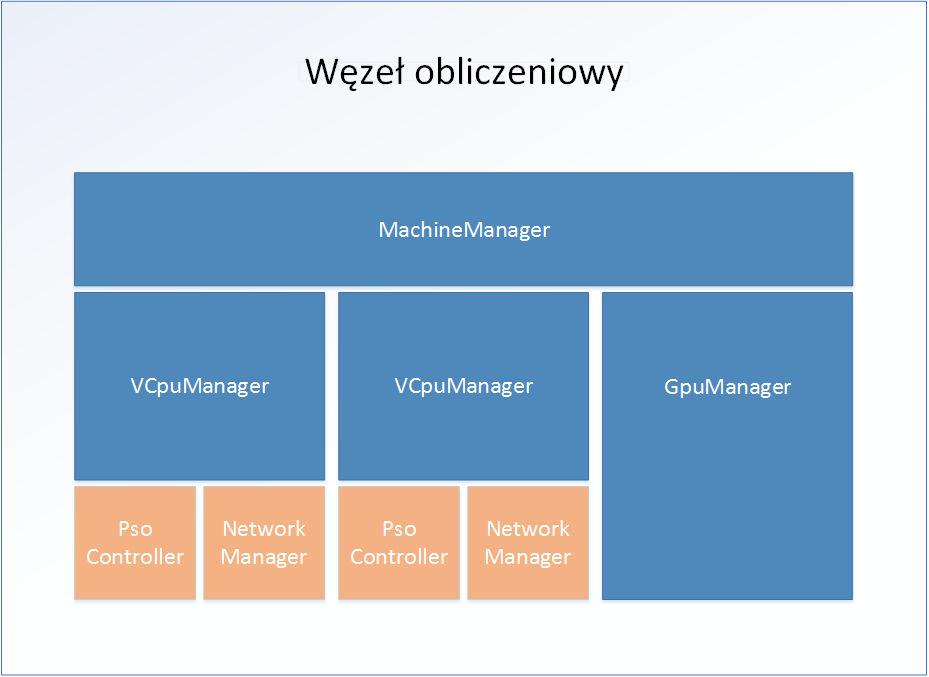
\includegraphics[width=1\textwidth,natwidth=610,natheight=642]{WezlaArch.png}
 \caption{Architektura węzła obliczeniowego}
\end{figure}

\subsection{MachineManager}
Klasa zarządzająca działaniem maszyny. Umożliwiająca wykorzystanie dostępnych zasobów - rozpoznanie liczby wątków procesora oraz obecność karty graficznej i jej kompatybilność z technologią CUDA. Jest obiektem zaimplementowanym według wzorca fasada, który jest odpowiedzialny za rozpoczęcie obliczeń alogrytmu oraz pobranie wyniku. Za pomocą metody \emph{Register} możemy podłączyć maszynę do klastra obliczeniowego. Odwołuje się do dwóch klas VCpuManager oraz GpuManager, za których pomocą udostępnia powyższe funkcjonalności.
Korzysta z wielu VCpuManager'ów, z których każdy odpowiada pojednyczemu z wątkowi procesora. Domyślnie, tworzone jest tyle wątków, ile dostępnych procesorów posiada komputer. Programista, może jednak ustawić własną liczbę wątków.

\subsection{VCpuManager}
Klasa odpowiedzialna za uruchomienie obliczeń algorytmu na pojedynczym wątku procesora oraz połączenie z pozostałymi węzłami klastra. Węzłem nazywamy tutaj pojedynczy wątek procesora, reprezentujący obliczenia jednego roju cząstek. W celu oddzielenia infrastruktury sieciowej od logiki dotyczącej algorytmu PSO wykorzystuje ona interfejsy \emph{IPsoManager}, który zarządza warstwą logiczną klastra PSO oraz \emph{INodeService} odpowiedzialny za komunikację pomiędzy węzłami korzystający z technologii WCF. \emph{VCpuManager} rozpoczyna oraz kończy nasłuchiwanie na portach TCP. Stosując wzorzec obserwator zaimplementowany za pomocą funkcjonalności wydarzeń języka C\# obsługuje nowe zapytania przesyłane przez pozostałe węzły zbudowanego klastra.


\subsection{PsoController}
Klasa, która na podstawie przekazanych jej parametrów problemu oraz algorytmu rozpoczyna wykonanie obliczeń. Pozwala ona na sprawdzenie czy obecnie uruchomione są obliczenia. Konfiguracja algorytmu jest dokonana na podstawie parametrów przekazanyc przez klasę \emph{PsoParams}. Zawarte są w niej wszystkie informacje potrzebne do uruchomienia obliczeń:

\begin{itemize}
	\item Epsilon - dokładność obliczeń algorytmu
	\item FunctionParams - parametry funkcji celu: 
	
	\item Iterations - maksymalna liczba iteracji do przeprowadzenia na wątku CPU
	\item IterationsLimitCondition - wartość logiczna stanowiąca o zatrzymaniu algorytm po wykonaniu danej liczby iteracji
	\item ParticleIterationsToRestart - liczba iteracji bez poprawy położenia cząstki, po której cząstka zostanie zrestartowana, czyli jej położenie zostanie wylosowane, a najlepsza wartość cząstki będzie równa nowemu położeniu
	\item Particles - lista typów oraz ilości cząstek do wykorzystania
	\item PsoIterationsToRestart - liczba iteracji bez poprawy najlepszego wyniku wszystkich cząstek, po której zakończone zostanie działanie algorytmu
	\item TargetValue - wartość ekstremalna funkcji celu, do której dąży wynik algorytmu
	\item TargetValueCondition - wartość logiczna stanowiąca, czy zatrzymać algorytm po zbliżeniu się na odległość \emph{Epsilon} od \emph{TargetValue}
\end{itemize}
\section{Implementacja algorytmu}
Algorytm PSO w wariencie uruchamianym na CPU został przez nas zaimplementowany w jęzku C\#, co różni się od wstępnych założeń projektu, w których zakładaliśmy jego implementację w języku C++ oraz opakowanie go klasą w technologii .NET . Początkowo algorytm został napisany zgodnie z założeniami systemu - algorytm w języku C++ natomiast jego opakowanie w języku C++/CLI. Jest to język oparty na C++ pozwalający na proste połączenie kodu natywnego C++ z kodem zarządzanym platformy .NET. Rozwiązanie takie było wystarczające dla tego modułu systemu, lecz okazało się być nadmierną komplikacją w budowie klastra oraz wykorzystaniu benchmarków BBOB.\\
W pierwszym przypadku utrudnieniem była konieczność użycia klas udostępniających usługi WCF w natywnym kodzie C++, aby  z perspektywy cząstek komunikacja między zdalnymi węzłami przebiegała w sposób jednolity do interakcji z cząstkami lokalnymi, następnie opakowanie tych cząstek w klasy języka C\# .\\
Drugi przypadek konfliktował z jednym z założeń, na podstawie którego programista mógł definiować funkcje celu w języku C\#. W celu spełnienia tego przekazywaliśmy funkcje z maszyny wirtualnej .NET do środowiska natywnego w celu ich wywołania przez cząstki. Wykorzystanie benchmarków wymagałoby dodatkowo odwrotnego opakowywania funkcji napisanych w C i rodziło dodatkowe komplikacje z odtwarzaniem funkcji dla zdalnych węzłów.
\subsection{Algorytm}
Zaimplementowanie algorytmu w języku C\# rozwiązało powyższe problemy oraz dodatkowo umożliwiło dużo przejrzystsze przekazywanie parametrów algorytmu oraz ułatwiało rozszerzanie algorytmu o nowe typy cząstek.
Sam algorytm stworzony został przez nas w taki sposób, aby był jak najbardziej generyczny ze względu na rodzaj cząstek, przez co jest odpowiedzialny jedynie za przeprowadzenie odpowiednich kroków algorytmu, których dokładna implementacja zawarta jest w cząstkach. W pętli sprawdzane są warunki stopu oraz liczone iteracje od ostatniej poprawy algorytmu, jeśli któryś z warunków zostanie spełniony, lub iteracje bez poprawy osiągną ustalony limit działanie algorytmu zostaje przerwane.

\lstset{style=sharpc}
\begin{lstlisting}[frame=single]
public IState<double[],double[]> Run(CancellationToken token)
{
	foreach(var particle in _particles)
	{
		var j = randomParticleIndex();	      
		particle.Transpose(_fitnessFunction);
	    particle.UpdateNeighborhood(_particles);
		particle.InitializeVelocity(_particles[j]);
	}
	var _currentBest = GetCurrentBest();
	_globalBest = new ParticleState(_currentBest.Location,
	_currentBest.FitnessValue);
	while (_conditionCheck())
	{
		foreach (var particle in _particles)
		{
	    	particle.Transpose(_fitnessFunction);
	    }
		foreach (var particle in _particles)
	    {
			particle.UpdateVelocity(_globalBest);
		}
	}
	return _fitnessFunction.BestEvaluation;
}
\end{lstlisting}


\subsection{Cząstka PSO}
W naszym systemie cząstki są implementacją interfejsu IParticle, który zawiera właściwości potrzebne do identyfikacji cząstki, określenia jej położenia obecnego i najlepszego dotychczas odwiedzonego oraz metody   aktualizujące sąsiedztwo cząstki, jej prędkość i położenie. Od implementacji cząstek zależy topologia roju oraz sposób w jaki poruszają się po przestrzeni poszukiwań. 

\subsubsection{StandardParticle}
W celu dokładniejszego opisu cząstki przestawimy przykładową cząstkę zbudowaną zgodnie z założeniami SPSO.%Czy aby napewno
Rozszerza ona abstrakcyjną klasę Particle, która zawiera elementy wspólne pomiędzy różnymi wersjami cząstek. Topologia jest ustalana poprzez funkcję UpdateNeighborhood, która wybiera sąsiadów, z którymi się komunikuje dana cząstka.
\lstset{style=sharpc}
\begin{lstlisting}[frame=single]
public override void UpdateNeighborhood(IParticle[] allParticles)
{
	Neighborhood = allParticles
	.Where(particle => particle.Id != Id)
	.ToArray();
}
\end{lstlisting}

Funkcja UpdateVelocity aktualizuje prędkość cząstki uwzględniając najlepsze położenia swoje oraz cząstek sąsiednich. W danym przykładzie, aby uzyskać wzrost wydajności algorytmu pojedyncza cząstka nie szuka najlepszej pozycji sąsiadów tylko otrzymuje globalną najlepszą wartość jako parametr funkcji. Jest to wartość identyczna z najlepszą wartością sąsiedztwa cząstki, gdyż w tym przypadku jest nim cały rój.

\lstset{style=sharpc}
\begin{lstlisting}[frame=single]

        public override void UpdateVelocity(IState<double[], double[]> globalBest)
        {
            // 1.  get vectors to personal and global best
            var toPersonalBest = Metric
            .VectorBetween(CurrentState.Location, PersonalBest.Location);
            
            var toGlobalBest = 
            Metric
            .VectorBetween(CurrentState.Location, globalBest.Location);

            var phi1 = RandomGenerator.RandomVector(CurrentState.Location.Length, 0, Constants.PHI);
            var phi2 = RandomGenerator.RandomVector(CurrentState.Location.Length, 0, Constants.PHI);

            // 2. multiply velocity by Omega and add toGlobalBest and toPersonalBest
            Velocity = Velocity.Select((v, i) => v * Constants.OMEGA + phi1[i] * toGlobalBest[i] + phi2[i] * toPersonalBest[i]).ToArray();
        }

\end{lstlisting}

Funkcja Transpose jest odziedziczona z klasy Particle, ponieważ jest wspólna dla stosowanych przez nas typów cząstek. Zmienia ona obecne położenie cząstki licząc przy tym liczbę iteracji bez poprawy wartości funkcji celu. Jeśli przekroczy ona ustalony w konfiguracji algorytmu limit, cząstka jest restartowana, czyli losowane jest jej położenie początkowe oraz zapominane najlepsze dotychczas rozwiązanie.

\lstset{style=sharpc}
\begin{lstlisting}[frame=single]
public virtual void Transpose(IFitnessFunction<double[], double[]> function)
        {
            double[] newLocation;
            if (_sinceLastImprovement == _iterationsToRestart)
            {
                newLocation = randomLocation()
                _sinceLastImprovement = 0;
            }
            else
            {
                newLocation = GetClampedLocation(CurrentState.Location + Velocity);
            }
            var newVal = function.Evaluate(newLocation);
            var oldBest = PersonalBest;
            CurrentState = new ParticleState(newLocation, newVal);

            if (Optimization.IsBetter(newVal, PersonalBest.FitnessValue) < 0)
            {
                PersonalBest = CurrentState;
                _sinceLastImprovement = 0;
            }
            else
            {
                _sinceLastImprovement++;
            }
        }
\end{lstlisting}

\subsection{Funkcja celu}
Funkcje celu są obiektami implementującymi interfejs IFitnessFunction. Udostępniają one liczbę przeprowadzonych ewaluacji funkcji, najlepszą ewaluację oraz informacje o wymiarze przestrzeni poszukiwań i wartości funkcji. Funkcje są tworzone przez fabrykę funkcji FunctionsFactory na podstawie przekazanych do niej parametrów. W celu stworzenia odpowiedniej funkcji klient musi przekazać odpowiednią nazwę funkcji. Jest to szczególnie ważne w przypadku funkcji benchamrkowych, gdyż w nazwie zakodowany jest rodzaj funkcji oraz jej odpowiednia instancja. Dodatkowo fabryka funkcji umożliwia zapisanie danej funkcji w cache'u. Konieczność zastosowania pamięci tymczasowej była wynikiem integracji systemu z biblioteką COCO, która wymagała użycia jednej instancji funkcji celu w całym systemie.

\section{Klaster i komunikacja między węzłami}
Komunikacja między węzłami przebiega na dwóch opisanych poniżej poziomach. 

\subsection{Komunikacja na poziomie algorytmu}
Jednym z nich jest komunikacja na poziomie rojów cząstek przekazujących sobie informacje o dotychczas najlepszym odnalezionym położeniu. Połączenia pomiędzy węzłami w tej warstwie zarządzane są przez interfejs IPsoManager, który posiadając informacje o połączonych jednostkach definiuje sąsiedztwa pomiędzy nimi. W przypadku naszego klastra implementuje on strukturę pierścienia, w której każdy węzeł posiada dwóch sąsiadów. Połączenia pomiędzy rojami działającymi wewnątrz jednej maszyny, ale korzystające z różnych wątków procesora przebiegają w ten sam sposób co połączenia między różnymi maszynami. Wszystkie wątki wszystkich maszyn tworzą jeden pierścień. Komunikacja pomiędzy rojami jest dwustronna. Z perspektywy cząstek wewnątrz roju, sąsiedni rój jest reprezentowany przez cząstkę proxy. Ona sama nie jest częścią algorytmu (nie wykonuje ewaluacji funkcji celu), przekazuje jedynie najlepsze znane położenie zwykłej cząstki z nią zespolonej pomiędzy rojami. Lokalnie podaje najlepszy wynik znany cząstce proxy z roju sąsiedniego, natomiast do niej przekazuje informacje od lokalnej cząstki. Poza informacjami przekazywanymi przez cząstki proxy, po zakończeniu obliczeń każdy z węzłów rozsyła do pozostałych argument, dla którego wartość funkcji celu jest najbardziej zbliżona do poszukiwanego optimum.


\subsection{Infrastruktura klastra}



Klaster obliczeniowy jest oparty na topologii pełnej siatki, w której każdy węzeł połączony jest z wszystkimi pozostałymi. Każdy z wątków procesora jest dołączany do sieci niezależnie od pozostałych. Komunikacja realizowana jest za pomocą usług WCF korzystających z protokołu sieciowego TCP. Obliczenia są niezależne od połączeń pomiędzy węzłami klastra, dzięki czemu po awarii jednego z nich obliczenia nie są przerywane, a topologia sąsiedztwa rojów algorytmu PSO jest dostosowywana do dostępnych w danym momencie węzłów. Każdy z węzłów jest równoważny wszystkim pozostałym, to znaczy nie istnieje centralny serwer zarządzający pracą sieci, dzięki czemu obliczenia mogą być zapoczątkowane przez dowolny z nich. 

\begin{figure}[H]
    \centering
 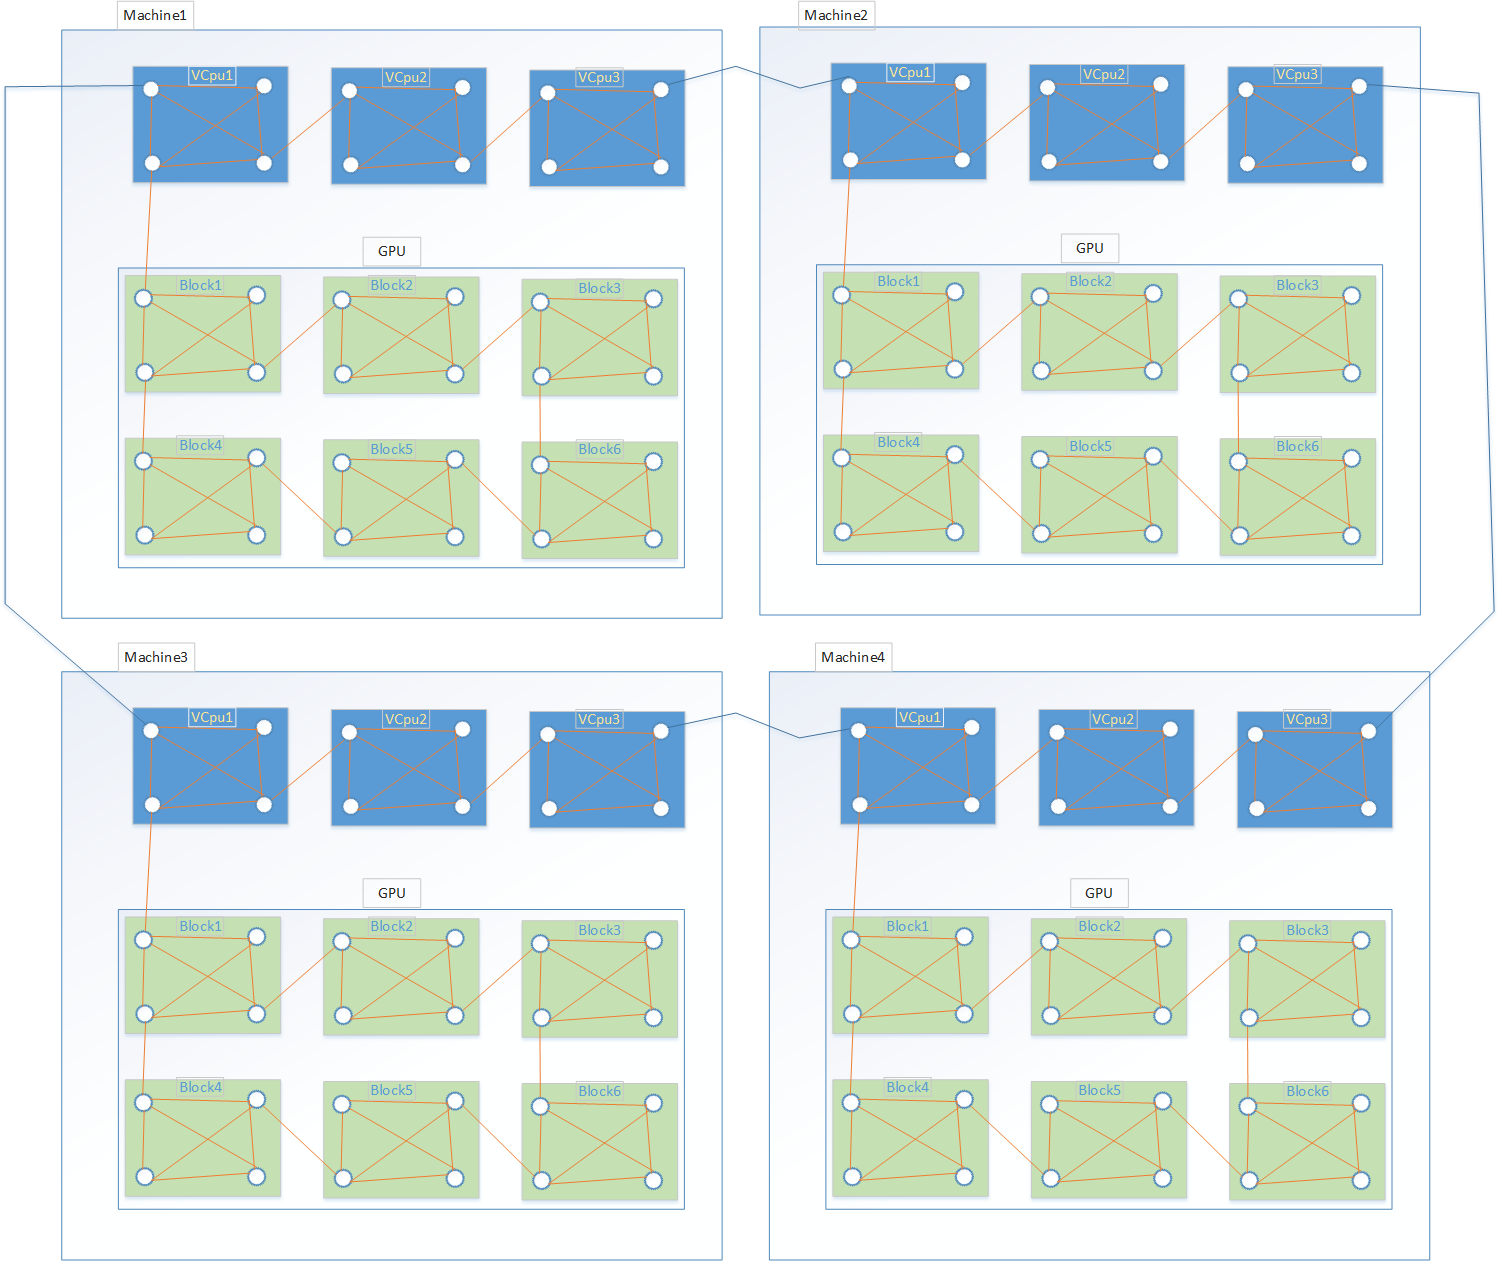
\includegraphics[width=1\textwidth,natwidth=610,natheight=642]{wholeCluster.png}
 \caption{Infrastuktura klastra}
\end{figure}

\section{Obliczenia na procesorze graficznym}
\subsection{Krótkie wprowadzenie do architektury CUDA}
%[Prosty opis bloków, wątków]
Opis części programu na GPU wymaga krótkiego wprowadzenia do organizacji wątków i pamięci w architekturze CUDA.

Podstawową jednostką obliczeniową 
%[to chyba niezbyt dobre określenie] 
w architekturze CUDA jest pojedynczy wątek GPU. Dzięki dostępowi do tysięcy wątków na procesorze graficznym możliwe jest stosowanie modelu SIMT (Single Instruction Multiple Threads). Każdy wątek ma dostęp do swojej lokalnej pamięci wątku. \\
Wątki zorganizowane są w wielowymiarowe bloki wątków. W zależności od wersji architektury, blok może zawierać 512 lub 1024 wątki. Poza grupowaniem wątków każdy blok wątków ma swój segment pamięci zwany pamięcią dzieloną bloku. Dostęp do tej pamięci jest dużo szybszy niż do pamięci globalnej, do której dostęp ma dowolny wątek obliczeniowy. \cite{CudaProgGuide}

\subsection{Implementacja algorytmu dla procesora graficznego}

Architektura części naszego programu odpowiadającej za obliczenia na GPU jest inspirowana pracami wspomnianymi powyżej. \cite{PsoCuda} \cite{GpuBasedPso} Całość opiera się na topologii pierścienia.

Rój cząstek na GPU działa w synchronizacji z rojem na CPU poprzez wyszczególnienie po obu stronach cząstek odpowiedzialnych za przekazywanie swojej pozycji w roju na danej jednostce obliczeniowej rojowi na drugim procesorze (czyli pośrednio przekazuje pozycję własnego roju). Odnosząc się do topologii pierścienia, można wyobrazić to sobie jako most łączący 2 pierścienie.

Dalej, rój na GPU składa się z mniejszych rojów działających w obrębie bloków. Każdy z mniejszych rojów komunikuje się z dwoma sąsiednimi rojami, tworząc pierścień. Komunikacja odbywa się analogicznie jak w przypadku komunikacji z CPU - dla każdego sąsiedztwa w bloku wybierana jest cząstka służąca do przekazywania swojej pozycji (czyli pośrednio pozycji roju).

Podstawową jednostką w ramach roju na GPU są cząstki w rojach zorganizowanych w blokach. Każdy wątek w bloku odpowiada jednej cząstce w roju. Tak jak w poprzednim przypadku, tu również cząstki zorganizowane są w pierścień.

Taka organizacja cząstek pozwala na zmaksymalizowanie zużycia mocy obliczeniowej GPU - liczba cząstek w ogólnym roju odpowiada liczbie dostępnych wątków. Topologia pierścienia pozwala na ograniczenie potrzeby komunikacji międzywątkowej dzięki stałemu zestawowi dwóch sąsiadów. Organizacja mniejszych rojów w blokach wątków umożliwia korzystanie ze znacznie szybszej pamięci dzielonej.

\subsection{Komunikacja między procesorami obliczeniowymi}
 Celem implementacji algorytmu dla procesorów graficznych było współgranie obliczeń na CPU i GPU. Roje z obu jednostek obliczeniowych tworzą jeden większy rój, dzięki temu szybciej zbiegający algorytm na GPU ma szansę na nakierowanie roju CPU w dobrym kierunku.
 
 Komunikacja odbywa się w sposób niewidoczny dla samego algorytmu PSO poprzez specjalną cząstkę obecną zarówno w roju GPU i CPU. Cząstka ta przy zapytaniu o jej stan przez inną cząstkę z roju CPU odpowiada stanem wybranej cząstki z roju na GPU (analogicznie w przypadku zapytania ze strony GPU).       
 
 Synchronizacja stanów odbywa się co krok algorytmu na GPU. Dzieje się to w sposób przezroczysty dla algorytmu na CPU, ale konieczność pobrania stanu cząstki z pamięci graficznej wymusza drobną modyfikacje algorytmu na GPU.
 
 \subsection{Szczegóły implementacyjne}
Zestaw narzędzi CUDA udostępnia rozszerzenia jedynie dla języków C i C++. W celu integracji z pozostałą częścią systemu użyta została biblioteka ManagedCUDA, umożliwiająca łatwą kooperację środowisk .NET i CUDA.

Obliczenia na procesorze graficznym zarządzane są przez osobny wątek działający równolegle do algorytmu działającego na CPU. Wątek ten kontroluje inicjalizację środowiska, wykonanie i zakończenie algorytmu oraz komunikację między rojami GPU i CPU. 
 
 Na część natywną, odpowiadającą za działanie algorytmu na procesorze graficznym, składają się części algorytmu PSO, wywoływane przez wątek zarządzający, oraz funkcje używane do benchmarkowania.
 
\chapter{Platforma COCO}

\section{Testowanie algorytmów optymalizacyjnych}
Jednym z celów naszej pracy było przetestowanie jakości implementacji algorytmu PSO na stworzonym przez nas klastrze obliczeniowym. Do tego zadania postanowiliśmy wybrać platformę COCO \cite{Coco}.

Benchmarkowanie algorytmów optymalizacyjnych polega w skrócie na uruchomieniu algorytmu na przygotowanym wcześniej zbiorze problemów i zebraniu oraz przedstawieniu wyników. Nie jest to jednak tak trywialne zadanie, na jakie mogłoby wyglądać na pierwszy rzut oka m.in. ze względu na częstą trudność w dokładnej interpretacji otrzymanych wyników czy też porównaniu ich z innymi.

Odpowiedzią na te trudności jest ,,COCO framework'' umożliwiający zautomatyzowanie procedury benchmarkowania algorytmów optymalizacyjnych. Ideą przyświecającą twórcom COCO było stworzenie środowiska zapewniającego wszystkie niezbędne do przeprowadzenie testów funkcjonalności oraz możliwość porównania danych i wyników zebranych przez różne zespoły uczonych na przestrzeni lat używających tego framewokra.

%[why coco]

Funkcje do benchmarkowania, których używa COCO są jawne dla użytkownika, jednakże sam algorytm, który poddajemy testom, nie ma o nich żadnej wiedzy (działają na zasadzie black-box). Lista wszystkich funkcji używanych przez COCO dostępna jest w \cite{Coco}, jednakże my ograniczyliśmy się do pierwszych 24 funkcji (funkcje bez szumu).
Funkcje te są wybrane w ten sposób, aby dało się w jasny sposób zinterpretować na nich działanie algorytmu optymalizacyjnego. Dodatkowo nie posiadają one żadnych sztucznych regularności, które mogłyby zostać wykorzystane przez algorytm oraz są skalowalne ze względu na wymiar.


Co bardzo istotne, cały framework używa tylko jednej miary jakości algorytmu – tzw. runtime, czyli liczby ewaluacji funkcji celu potrzebnej do osiągnięcia zadanego wyniku, czyli znalezienia wartości funkcji celu odpowiednio bliskiej wartości optymalnej. Zalety takiego podejścia są opisane w \cite{CocoPlatform}. Dodatkowo nie zakłada się ustalonego z góry maksymalnego budżetu, określonego liczbą ewaluacji funkcji celu - testy są ,,budget free''.

COCO framework składa się z zestawu benchmarków napisanych w języku C wraz z modułami odpowiedzialnymi za zbieranie (logowanie) wyników, ich obróbkę (skrypty Python przygotowujące odpowiednie wykresy) oraz prezentację danych (dokumenty html oraz pliki pdf generowane na podstawie przygotowanych szablonów LaTeX). Dodatkowo twórcy frameworka przygotowali interfejsy w językach C/C++, Java, Matlab/Octave, Python (stan w grudniu 2016) zapewniające obsługiwanie napisanych przez użytkownika algorytmów optymalizacyjnych w wymienionych językach. Niestety w chwili pisania niniejszej pracy, nie był dostępny oficjalny interfejs do języka C\#, dlatego też zmuszeni byliśmy stworzyć własny.

\section{Wrapper}

Stworzony przez nas wrapper miał za zadanie umożliwić wywołanie funkcji biblioteki COCO (CocoLibrary.c) napisanych w języku C z poziomu naszej aplikacji w języku C\#. Przy jego tworzeniu wzorowaliśmy się na dostępnym wrapperze dla języka Java wykorzystującym Java Native Interface (JNI), czyli framework umożliwiający komunikację z kodem napisanym w C/C++. 


Pierwszym zadaniem było utworzenie klas języka C\# odpowiadających strukturom języka C, które były wykorzystywane w bibliotece COCO. Te klasy, to:

\textbf{Problem} - odpowiada strukturze \textit{coco\_problem\_t} i zawierająca dane konkretnego problemu optymalizacyjnego.\\
\textbf{Suite} - odpowiada strukturze \textit{coco\_suite\_t} i odpowiada całemu zestawowi problemów optymalizacyjnych.\\
\textbf{Observer} - odpowiada strukturze \textit{coco\_observer\_t}, która służy do zbierania danych w czasie wykonywania testów.\\
\textbf{Benchmark} - klasa opakowująca, zawierająca w sobie obiekt klasy \textbf{Suite} oraz obiekt klasy \textbf{Observer}, umożliwiająca pobranie kolejnego problemu optymalizacyjnego z zestawu.\\

Klasy te stanowią interfejs benchmarku dla naszego programu - tworzone oraz inicjalizowane są w głównej pętli procedury testującej.

Między powyżej opisanymi obiektami a funkcjami z \textit{CocoLibrary.c} pośredniczy jeszcze jedna warstwa, będąca prawdziwym wrapperem i zamknięta w klasie \textbf{CocoLibraryWrapper}.

\subsection{Eksport\textbackslash import funkcji z języka C}

Jedną z części klasy CocoLibraryWrapper stanowią zaimportowane funkcje z \textit{CocoLibrary.c}. Import funkcji jest konieczny, aby móc wywoływać je z poziomu języka C\#. Na przykładzie jednej z funkcji zaprezentujemy sposób ich importu, który wymaga następującej deklaracji:\\

\begin{lstlisting}[frame=single]
[DllImport(
"CocoLibrary.dll", 
CallingConvention = CallingConvention.Cdecl)]

unsafe static extern char* 
coco_problem_get_name(struct_pointer_t problem);
\end{lstlisting}

Umożliwia ona import funkcji o sygnaturze

\begin{lstlisting}[frame=single]
const char *coco_problem_get_name(const coco_problem_t *problem)
\end{lstlisting}

znajdującej się w pliku \textit{CocoLibrary.c}. Jak widać, aby zaimportować funkcję, należy wskazać jej źródło (w tym przypadku bibliotekę \textit{CocoLibrary.dll}) oraz sposób wywołania (w tym przypadku Cdecl, czyli konwencja właściwa dla języka C). 

Dodatkowo importowana funkcja musi zostać opatrzona modyfikatorami \textit{unsafe} (umożliwiający korzystanie ze wskaźników w języku C\#) oraz \textit{extern} (wskazująca, że implementacja funkcji znajduje się w innym miejscu).

Sam import funkcji w naszej aplikacji nie wystarcza, aby uzyskać do nich dostęp. Konieczny był również ich eksport z samej biblioteki \textit{CocoLibrary.c}, aby po jej skompilowaniu do \textit{CocoLibrary.dll}, były one widoczne na zewnątrz. Eksport funkcji dokonuje się w następujący sposób:\\

\begin{lstlisting}[frame=single]
__declspec(dllexport) 
const char *coco_problem_get_name(const coco_problem_t *problem);
\end{lstlisting}

Zaimportowanych funkcji nie wywołujemy bezpośrednio, a za pomocą jeszcze jednej warstwy pośredniczącej, z której to korzystają już opisane wcześniej klasy \textbf{Problem}, \textbf{Suite}, \textbf{Observer} i \textbf{Benchmark}. Dodatkowa warstwa była konieczna, aby zapewnić, że funkcje eksportowane z \textit{CocoLibrary.dll} wywoływane będą we właściwy sposób, jak np.:

\begin{lstlisting}[frame=single]
public static unsafe String cocoProblemGetName(long problemPointer)
        {
            char* str = coco_problem_get_name(problemPointer);
            return Marshal.PtrToStringAnsi((IntPtr)str);
        }
\end{lstlisting}

gdzie należy dokonać odpowiedniego marshallingu argumentów

\subsection{Wykorzystanie wrappera}

Wrapper wykorzystany został w naszym programie oczywiście do uruchomienia zestawu testów benchmarka COCO. Inicjalizacja odpowiednich klas dokonywana jest w następujący sposób:

\begin{lstlisting}[frame=single]
var suite = new Suite("bbob", "year: 2016", "dimensions: " + dims);
var observer = new Observer("bbob", observerOptions);
var benchmark = new Benchmark(suite, observer);
\end{lstlisting}

zaś w głównej pętli programu kolejny problem do optymalizacji pobierany jest z obiektu klasy \textbf{Bechmark}:

\begin{lstlisting}[frame=single]
Problem = benchmark.getNextProblem()
\end{lstlisting}


\chapter{Testy}

\section{Wyniki testów}

Poniżej znajdują się wyniki testów naszej biblioteki przy użyciu platformy COCO. % oraz %niezależnych od niej testów czasowych.
Zestawiamy ze sobą z jednej strony wyniki otrzymane przy użyciu pojedynczego węzła obliczeniowego, zarówno z wykorzystaniem GPU, jak i bez niego, z drugiej zaś wyniki głównego węzła obliczeniowego klastra mającego do dyspozycji 2 i 4 jednostki obliczeniowe, a zatem mogącego wykonać około 2- i 4-krotnie większą liczbę ewaluacji funkcji, ale nie korzystającego z obliczeń na kartach graficznych. Porównanie rezultatów wskazuje lepsze jakościowo rozwiązanie korzystające z obliczeń równoległych. Dodatkowo porównujemy ze sobą wyniki działania węzła obliczeniowego korzystającego z roju standardowych cząstek z węzłem, którego połowa populacji stanowią cząstki naładowane (z opisanej wcześniej wersji algorytmu PSO). 
Jednym z usprawnień względem podstawowej wersji algorytmu, które wprowadziliśmy do naszego rozwiązania, aby poprawić jego jakość są restarty algorytmu, gdy najlepsze znalezione rozwiązanie nie poprawi się przez odpowiednio długą liczbę iteracji oraz analogiczne restarty pojedynczych cząstek, które w przypadku braku poprawy znalezionego osobistego optimum, rozpoczynają poszukiwania od nowa w losowym punkcie dziedziny. Wyznaczona eksperymentalnie liczba iteracji, po których następują restarty 40 i 100 iteracji dla, odpowiednio, restarów cząstki i restartów globalnych.
%coco na klastrze jest inne

%%%%%%%%%%%%%%%%%%%%%%%%%%%%%%%%%%%%%%%%%%%%%%%%%%%%%%%%%%%%%%
\subsection{Pojedynczy węzeł obliczeniowy}



\subsubsection{Rój złożony ze standardowych cząstek}
\begin{figure}[H]
    \centering
 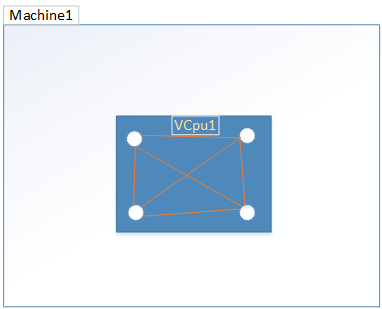
\includegraphics[width=1\textwidth,natwidth=410,natheight=442]{singleCPU.png}
 \caption{Pojedynczy węzeł obliczeniowy}
\end{figure}

\begin{figure}[H]
    \centering
 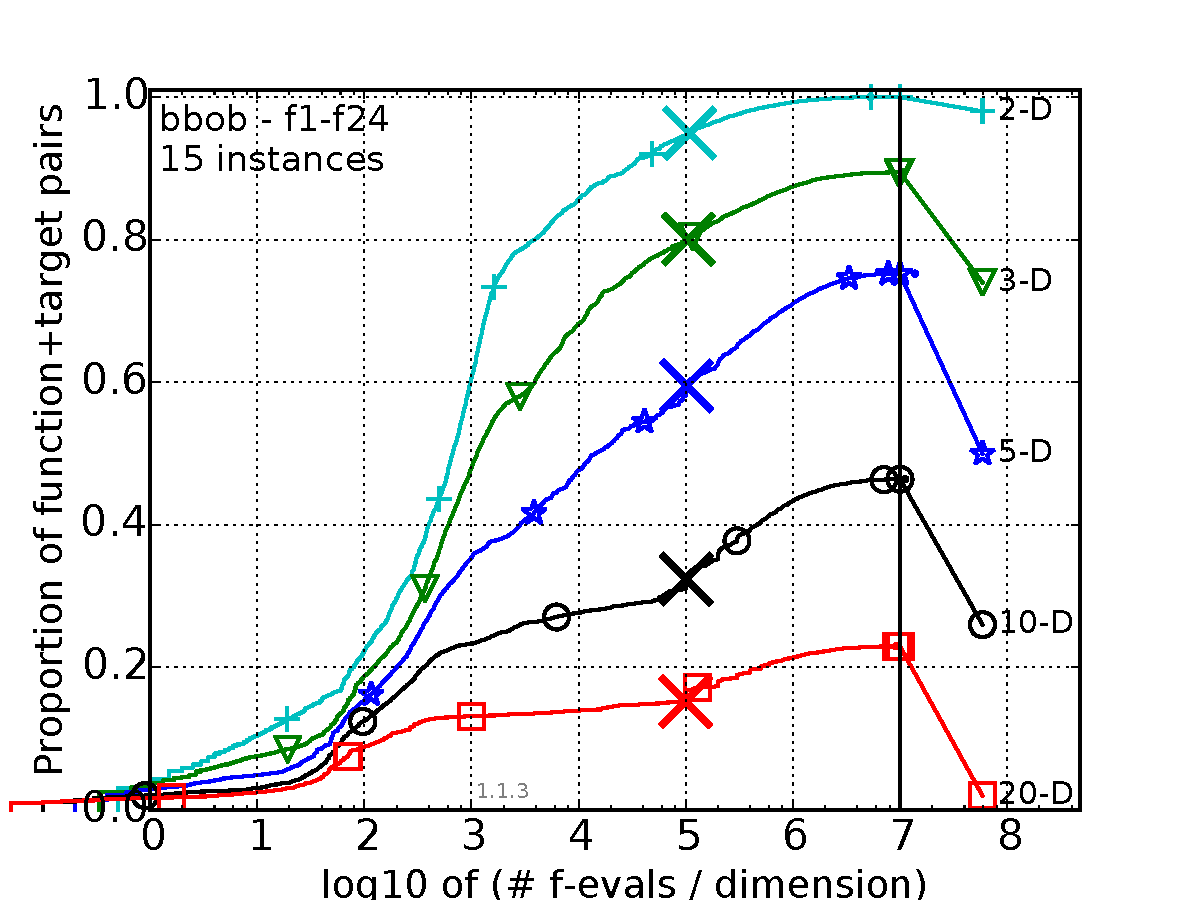
\includegraphics[width=1\textwidth,natwidth=610,natheight=642]{ogolne_single_st.pdf}
 \caption{Wyniki roju 40 standardowych cząstek}
\end{figure}

\subsubsection{Rój korzystający z GPU i złożony z cząstek standardowych i naładowanych}

\begin{figure}[H]
    \centering
 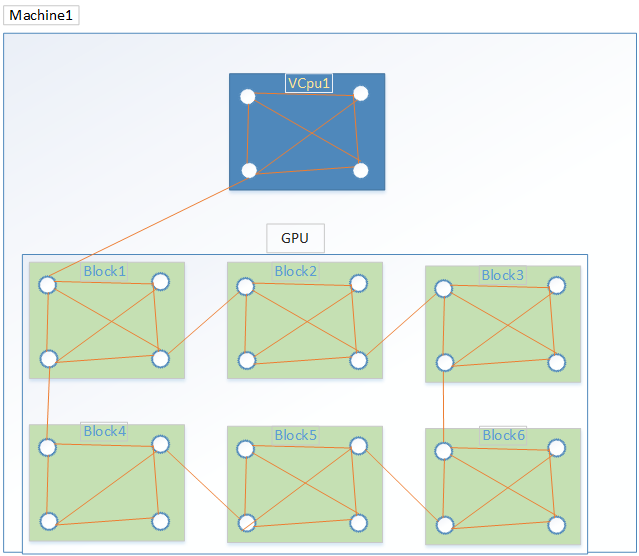
\includegraphics[width=1\textwidth,natwidth=610,natheight=642]{singleCpuGpu.png}
 \caption{Struktura węzła obliczneniowego. Rój złożony z 40 cząstek na CPU oraz 640 cząstek na GPU}
\end{figure}

\begin{figure}[H]
    \centering
 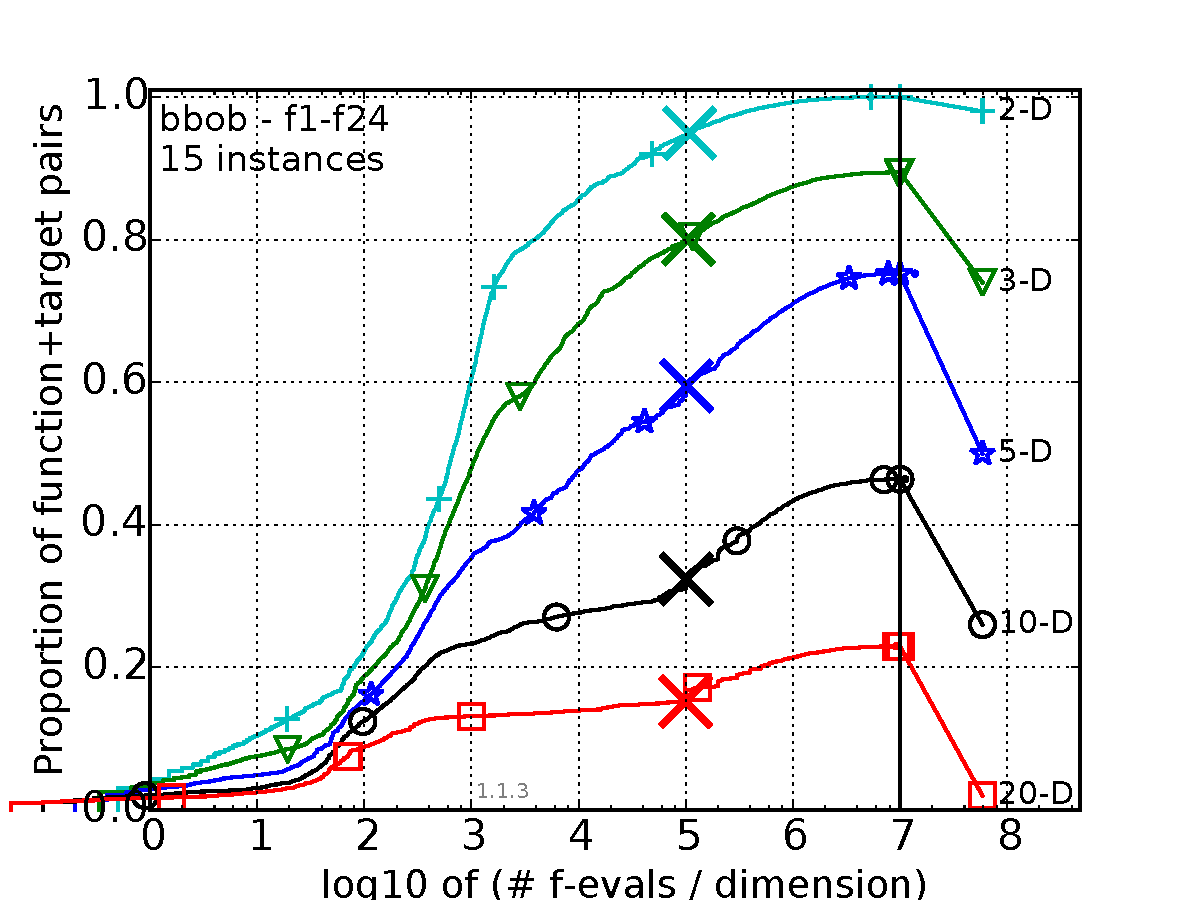
\includegraphics[width=1\textwidth,natwidth=610,natheight=642]{ogolne_single_st.pdf}
 \caption{Wyniki roju 20 cząstek standardowych i 20 cząstek naładowanych oraz 640 cząstek na GPU}
\end{figure}

%%%%%%%%%%%%%%%%%%%%%%%%%%%%%%%%%%%%%%%%%%%%%%%%%%%%%%%%%%%%%%%%%%%

\subsection{Klaster}

\subsubsection{Struktura klastra testowego}

\begin{figure}[H]
    \centering
 \includegraphics[width=1\textwidth,natwidth=610,natheight=642]{klasterBbobNoGpu.png}
 \caption{Struktura klastra testowego}
\end{figure}

\subsubsection{Klaster złożony z 2 węzłów obliczeniowych}

\begin{figure}[H]
    \centering
 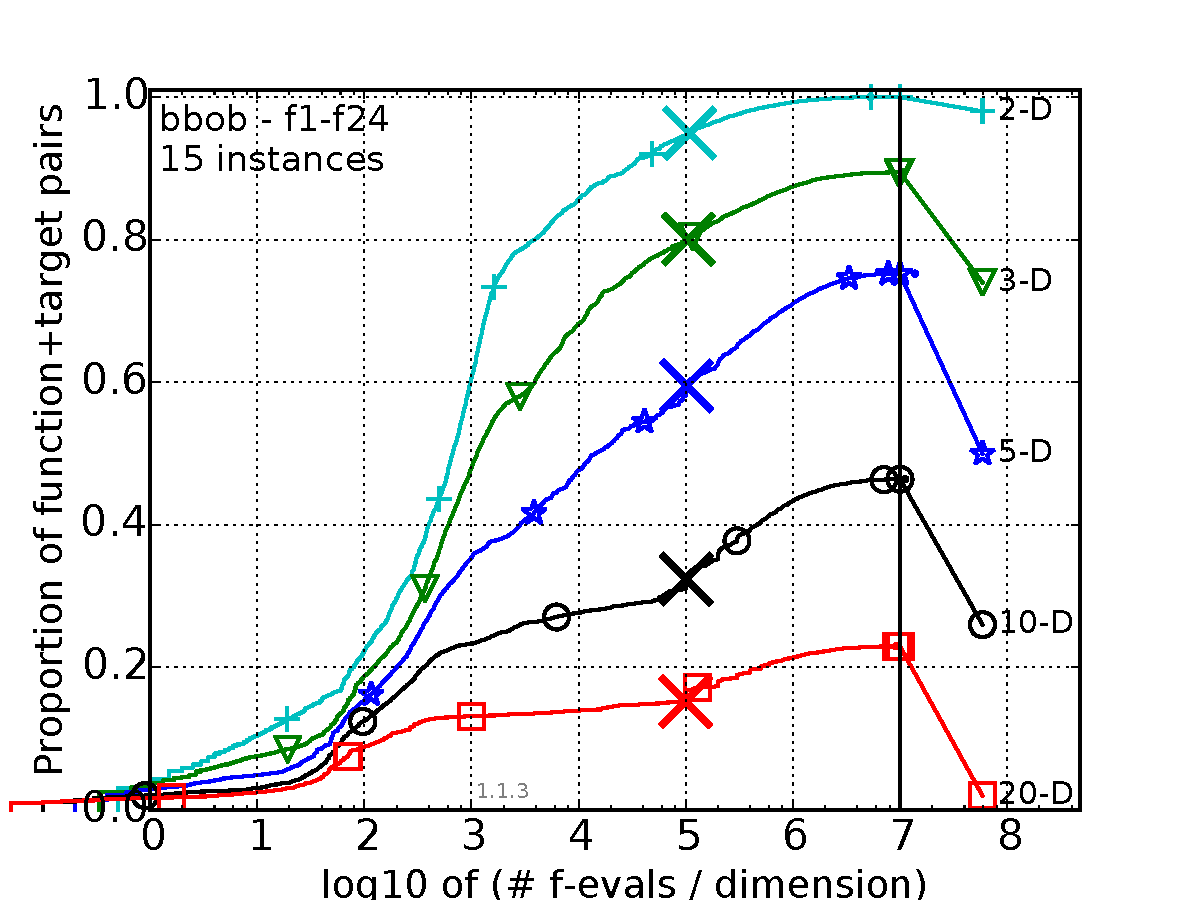
\includegraphics[width=1\textwidth,natwidth=610,natheight=642]{ogolne_single_st.pdf}
 \caption{Wyniki klastra z 2 węzłami obliczeniowymi}
\end{figure}

\subsubsection{Klaster złożony z 4 węzłów obliczeniowych}

\begin{figure}[H]
    \centering
 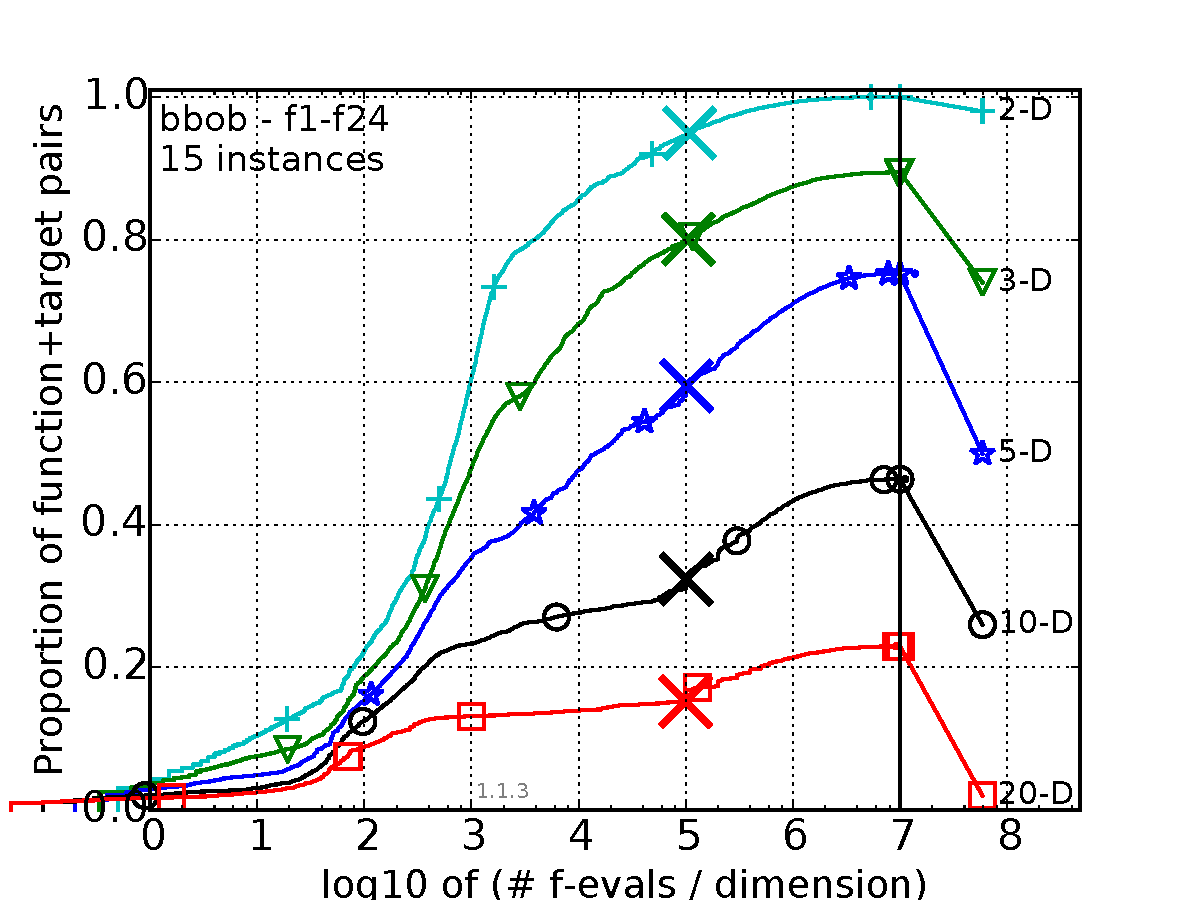
\includegraphics[width=1\textwidth,natwidth=610,natheight=642]{ogolne_single_st.pdf}
 \caption{Wyniki klastra z 4 węzłami obliczeniowymi}
\end{figure}


\section{Interpretacja wyników}

Otrzymane wyniki standardowej wersji PSO na pojedynczym węźle obliczeniowym są zgodne z oczekiwaniami - algorytm radzi sobie dobrze z prostymi funkcjami, takimi jak Linear Slope i szybko znajduje optimum z dużą dokładnością, jednakże dla funkcji trudnych, zwłaszcza w większym wymiarze, PSO osiąga bardzo nisko skuteczność.

Porównanie wyników standardowego PSO z wynikami uzyskanymi po zastąpieniu połowy cząstek roju cząstkami naładowanymi oraz użyciu pomocy GPU wskazuje niestety na jedynie niewielką poprawę działania, widoczną jedynie dla niektórych funkcji.

\begin{figure}[H]
    \centering
 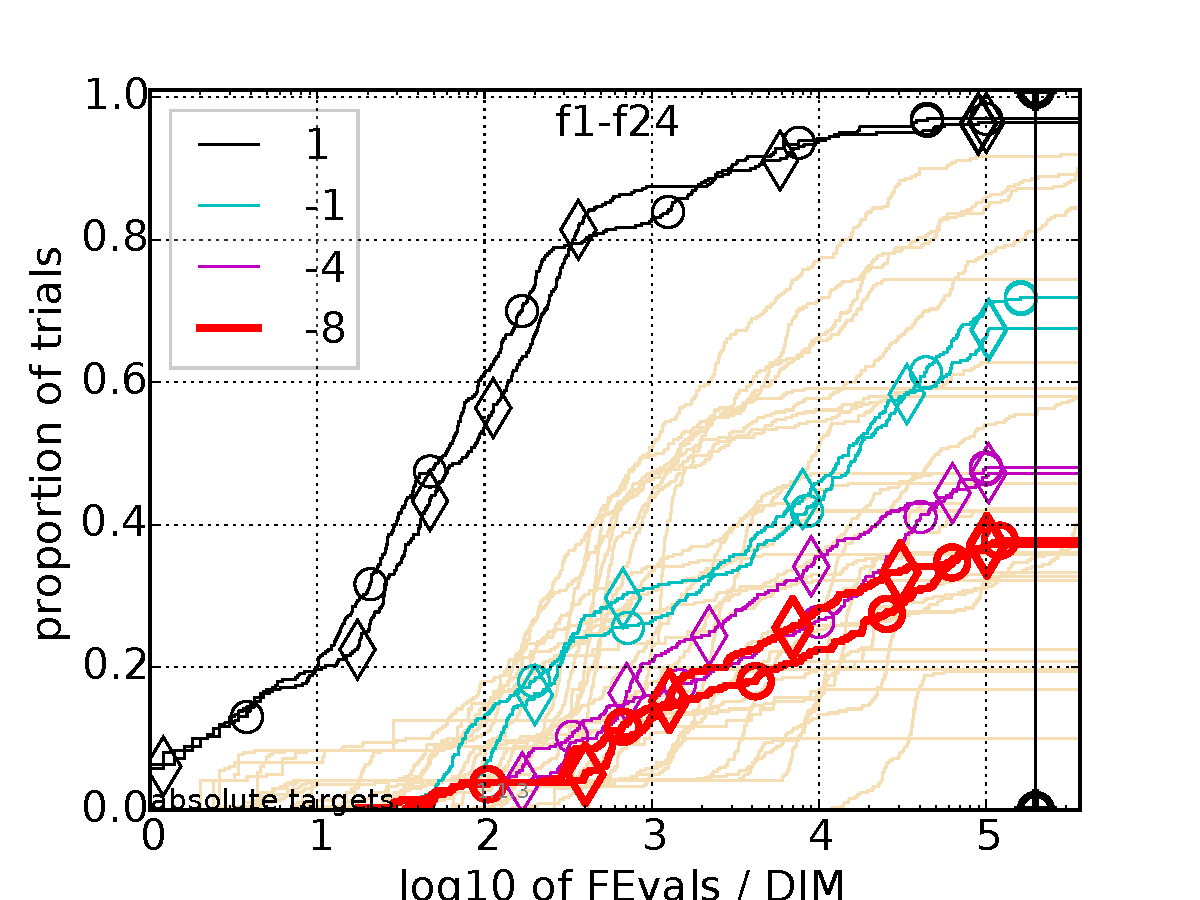
\includegraphics[width=1\textwidth,natwidth=610,natheight=642]{pprldistr_05D_noiselessall.pdf}
 \caption{Porównanie wersji z cząstkami naładowanymi i GPU (kółka) z wersją podstawową PSO}
\end{figure}

Znaczącą poprawę jakości działania algorytmu udało nam się uzyskać dopiero przy użyciu klastra obliczeniowego. Zgodnie z przewidywaniami stopień poprawy jest większy dla większej liczby węzłów obliczeniowych.

\begin{figure}[H]
    \centering
 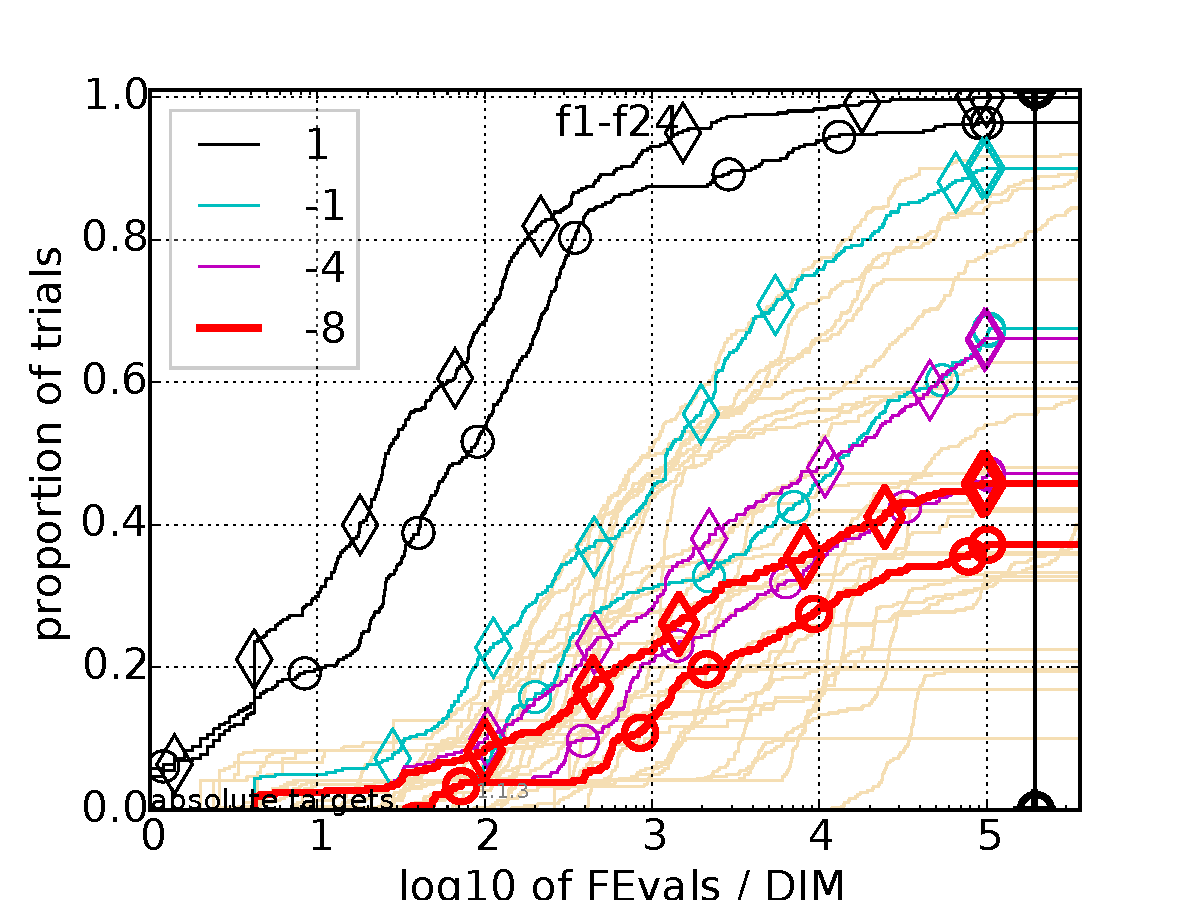
\includegraphics[width=1\textwidth,natwidth=610,natheight=642]{single_vs_cluster.pdf}
 \caption{Porównanie pojedynczego węzła obliczeniowego (kółka) z klaster o 4 węzłach}
\end{figure}


\chapter{Wymagania techniczne i instrukcja}

\section{Wymagania sprzętowe i programowe}

Do uruchomienia aplikacji niezbędny jest komputer z systemem operacyjnym Windows z
platformą .NET 4.5. W celu uruchomienia obliczeń na procesorze graficznym wymagana jest karta graficzna wspierająca wersję (compute capability) 2.0 architektury CUDA.

\section{Instrukcja użytkownika}

\subsection{Interfejs użytkownika}
Interfejs użytkownika pozwala na uruchomienie obliczeń dla jednej z zestawu predefiniowanych funkcji celu, włączając w to funkcje z benchmarku BBOB, używając zaimplementowanych typów algorytmu PSO. Umożliwia on odpowiednie dobranie parametrów funkcji celu oraz algorytmu. Za jego pomocą możliwym jest również utworzenie klastra obliczeniowego na wielu komputerach. Wybór oraz parametryzacja funkcji, algorytmu oraz konfiguracja klastra są kontrolowane przez odpowiednie pliki konfiguracyjne. 
\subsubsection{Klaster obliczeniowy}
Plik konfigurujący klaster obliczeniowy jest napisany w języku XML. Korzeniem dokumentu jest element o nazwe NodeParameters. 
Dziećmi elementu głównego są elementy:
\begin{enumerate}
	\item NrOfVCpu - wartość liczbowa definiująca liczbę węzłów, które zostaną utworzone przez program. Gdy przypiszemy mu wartość -1 obliczenia zostaną uruchomione na liczbie wątków dopasowanej do procesora.
	\item IsGpu - wartość logiczna włączająca/wyłączająca obliczenia na GPU
	\item Ip - adres interfejsu sieciowego maszyny, z którym będą mogły połączyć się pozostałe wątki klastra
	\item Ports - tablica integerów z numerami portów, na których nasłuchiwać będą usługi WCF
	\item PeerAddress - element zawierający adres węzła, do którego aplikacja powinna się podłączyć. Powinien zostać pominięty w przypadku, gdy użytkownik nie ma zamiaru łączyć się z innymi stacjami
\end{enumerate}
Przykładowy plik konfiguracyjny klastra:
\lstset{language=XML}
\begin{lstlisting}[frame=single]
<?xml version="1.0" encoding="utf-8"?>
<NodeParameters xmlns:xsi="http://www.w3.org/2001/XMLSchema-instance" xmlns:xsd="http://www.w3.org/2001/XMLSchema">
  <NrOfVCpu>1</NrOfVCpu>
  <IsGpu>false</IsGpu>
  <Ip>25.123.241.71</Ip>
  <Ports>
    <int>8000</int>
  </Ports>
  <PeerAddress>net.tcp://25.123.244.149:8000/NodeService</PeerAddress>
</NodeParameters>
\end{lstlisting}

\subsubsection{Algorytm PSO}
Plik konfigurujący algorytm PSO oraz funkcję celu również napisany jest w języku XML. Korzeniem dokumentu jest element o nazwe PsoParameters. 
Dziećmi elementu głównego są elementy:
\begin{enumerate}
	\item Particles - tablica definiująca liczbę oraz rodzaj cząstek użytych do obliczeń
	\item IterationsLimitCondition, Iterations - wartość logiczna określająca czy warunek stopu ze względu na liczbę iteracji powinien być zastosowany oraz liczba iteracji do wykonania
	\item TargetValueCondition, TargetValue, Epsilon - wartość logiczna określająca czy warunek stopu ze względu na osiągnięcie optimum powinien być zastosowany, optimum funkcji celu do wykonania oraz dokładność z jaką powinno być osiągnięte
	\item FunctionParameters - definiujące parametry funkcji celu. Dziećmi tego elementu są:
	\begin{enumerate}
		\item FitnessFunctionType - typ funkcji celu. Id funkcji w przypadku funkcji z benchmarku BBOB
		\item Dimension - wymiar funkcji
		\item Coefficients - współczynniki funkcji
		\item SearchSpace - tablica zawierająca dolną i górną granicę dziedziny poszukiwań
	\end{enumerate}

\end{enumerate}
\clearpage
Przykładowy plik konfiguracyjny algorytmu PSO:
\lstset{language=XML}
\begin{lstlisting}[frame=single]
<?xml version="1.0" encoding="utf-8"?>
<PsoParameters xmlns:xsi="http://www.w3.org/2001/XMLSchema-instance" xmlns:xsd="http://www.w3.org/2001/XMLSchema">
  <Particles>
    <ParticlesCount>
      <ParticleType>Standard</ParticleType>
      <Count>6</Count>
    </ParticlesCount>
  </Particles>
  <IterationsLimitCondition>true</IterationsLimitCondition>
  <Iterations>1000</Iterations>
  <TargetValueCondition>false</TargetValueCondition>
  <TargetValue>0</TargetValue>
  <Epsilon>0</Epsilon>
      <FunctionParameters>
        <FitnessFunctionType>quadratic</FitnessFunctionType>
        <Dimension>2</Dimension>
        <Coefficients>
          <double>1.0</double>
          <double>1.0</double>
        </Coefficients>
        <SearchSpace>
          <DimensionBound>
            <Min>-5</Min>
            <Max>5</Max>
          </DimensionBound>
    	  <DimensionBound>
            <Min>-5</Min>
            <Max>5</Max>
          </DimensionBound>
        </SearchSpace>
      </FunctionParameters>
</PsoParameters>
\end{lstlisting}

%-----------Koniec części zasadniczej-----------

\begin{thebibliography}{11}

%Evolving Objects

\bibitem{EObjGeneral} M. Keijzer, J. J. Merelo, G. Romero, M. Schoenauer, \emph{Evolving Objects: a general purpose evolutionary computation library}, http://geneura.ugr.es/~jmerelo/habilitacion2005/papers/53.pdf

\bibitem{EOlib} \emph{Evolving Objects homepage}, http://eodev.sourceforge.net/

%COCO

\bibitem{Coco} \emph{COCO homepage}, http://coco.gforge.inria.fr

\bibitem{CocoPlatform} N. Hansen, A. Auger, O. Mersmann, T. Tusar, D. Brockhoff, \emph{COCO: a platform for comparing continuous optimizers in a black-box setting}, https://arxiv.org/pdf/1603.08785.pdf

%%

\bibitem{NewPso} R. C. Eberhart, J. Kennedy, \emph{A new optimizer using particle swarm theory}, Proc. 6th Int. Symp. Micromachine Human Sci., Nagoya, Japan, 1995, pp. 39-43

\bibitem{Pso} J. Kennedy, R. C. Eberhart, \emph{Particle swarm Optimization}, Proc. IEEE Int. Conf. Neural Networks, 1995, pp. 1942-1948

\bibitem{SPso} Maurice Clerc, \emph{Standard particle swarm optimisation. From 2006 to 2011}, http://clerc.maurice.free.fr/pso/SPSO\_descriptions.pdf

\bibitem{PSO_2D_img} Randy Olson, \emph{Visualization of two dimensions of a NK fitness landscape}, 2013, URL https://commons.wikimedia.org/wiki/ \\ File:Visualization\_of\_two\_dimensions\_of\_a\_NK\_fitness\_landscape.png., [Online; dostęp grudzień 2016]

%z Comprehensive Learning PSO...

\bibitem{ComprLearnPso} J. J. Liang, A. K. Qin, P. N. Suganthan, S. Baskar, \emph{Comprehensive learning particle swarm optimizer for global optimization of multimodal functions}, IEEE Transactions on Evolutionary Computation, Vol. 10, No. 3, June 2006

\bibitem{ModPsoInertia} Y. Shi, R. C. Eberhart, \emph{A modified particle swarm optimizer}, Proc. IEEE Congr. Evol. Comput., 1998, pp. 69-73

\bibitem{ParamSelPso} Y. Shi, R. C. Eberhart, \emph{Parameter selection in particle swarm optimization}, Proc. 7th Conf. Evol. Programming, New York, 1998, pp. 591-600

\bibitem{PsoFuzzyInertia} Y. Shi, R. C. Eberhart, \emph{Particle swarm optimization with fuzzy adaptive inertia weight}, Proc. Workshop Particle Swarm Optimization, Indianapolis, IN, 2001, pp. 101-106

\bibitem{SelfOrgHPso} A. Ratnaweera, S. Halgamuge, H. Watson, \emph{Self-organizing hierarchical particle swarm optimizer with time varying accelerating coefficients}, IEEE Trans. Evol. Comput., vol. 8, pp. 240-255, Jun. 2004

\bibitem{VmaxPso} H. Y. Fan, Y. Shi, \emph{Study on Vmax of particle swarm optimization}, Proc. Workshop Particle Swarm Optimization, Indianapolis, IN, 2001

\bibitem{TopologyPso} J. Kennedy, \emph{Small worlds and mega-minds: Effects of neighborhood topology on particle swarm performance}, Proc. Congr. Evol. Comput., 1999, pp. 1931-1938

\bibitem{PopStructPso} J. Kennedy, R. Mendes, \emph{Population structure and particle swarm performance}, Proc. IEEE Congr. Evol. Comput., Honolulu, HI, 2002, pp. 1671-1676

\bibitem{PsoNeighOp} P. N. Suganthan, \emph{Particle swarm optimizer with neighborhood operator}, Proc. Congr. Evol. Comput., Washington, DC, 1999, pp. 1958-1962

\bibitem{MultiobjDynNeighPso} X. Hu, R. C. Eberhart, \emph{Multiobjective optimization using dynamic neighborhood particle swarm optimization}, Proc. Congr. Evol. Comput., Honolulu, HI, 2002, pp. 1677-1681

\bibitem{UPso} K. E. parsopoulos, M. N. Vrahatis, \emph{UPSO-A unified particle swarm optimization scheme}, Lecture Series on Computational Sciences, 2004, pp. 868-873

\bibitem{FullyInformedPso} R. Mendes, J. Kennedy, J. Neves, \emph{The fully informed particle swarm: Simpler, maybe better}, IEEE Trans. Evol. Comput., vol. 8, pp. 204-210, Jun. 2004

\bibitem{FitnessDistRatio} T. Peran, K. Veeramachaneni, C. K. Mohan, \emph{Fitness-distance-ratio based particle swarm optimization}, Proc. Swarm Intelligence Symp., 2003, pp. 174-181

\bibitem{SelectionPso} P. J. Angeline, \emph{Using selection to improve particle swarm optimization}, Proc. IEEE Congr. Evol. Comput., Anchorage, AK, 1998, pp. 84-89

\bibitem{HybridPsoBreedingSubpop} M. Lovbjerg, T. K. Rasmussen, T. Krink, \emph{Hybrid particle swarm optimizer with breeding and subpopulations}, Proc. Genetic Evol. Comput. Conf., 2001, pp. 469-476

\bibitem{EPso} V. Miranda, N. Fonseca, \emph{New evolutionary particle swarm algorithm (EPSO) applied to voltage/VAR control}, Proc. 14th Power Syst. Comput. Conf., Seville, Spain, 2002. [Online]. Available: http://www.pscc02.org/papers/s21pos.pdf

\bibitem{PsoCriticality} M. Lovbjerg, T. Krink, \emph{Extending particle swarm optimizers with self-organized criticality}, Proc. Congr. Evol. Comput., Honolulu, HI, 2002, pp. 1588-1593

\bibitem{CollisionAvoiding} T. M. Blackwell, P. J. Bentley, \emph{Don't push me! Collision-avoiding swarms}, Proc. IEEE Congr. Evol. Comput., Honolulu, HI, 2002, pp. 1691-1696

\bibitem{DissipativePso} X. Xie, W. Zhang, Z. Yang, \emph{A dissipative particle swarm optimization}, Proc. Congr. Evol. Comput., Honolulu, HI, 2002, pp. 1456-1461

\bibitem{ComputGlobOptPso} K. E. Parsopoulos, M. N. Vrahatis, \emph{On the computation of all global minimizers through particle swarm optimization}, IEEE Trans. Evol. Comput., vol. 8, pp. 211-224, Jun. 2004

%z Comparison of parallel PSO...

\bibitem{ComparisonParallelGpuPso} V. Roberge, M. Tarbouchi, \emph{Comparison of parallel particle swarm optimizers for graphical processing units and multicore processors}, International Journal of Computational Intelligence and Applications, Vol. 12 No. 1 (2013)

\bibitem{ComparGpuPso} G. A. Laguna-Sanchez, M. Olguin-Carbajal, N. Cruz-Cortes, R. Barron-Fernandez, J. Alvarez-Cedillo, \emph{Comparative study of parallel variants for a particle swarm optimization algorithm implemented on a multithreading GPU}, J. Appl. Res. Technol. 7(3) (2010) 292-309

\bibitem{BlockOccupancyGpu} M. Cardenas-Montes, M. Vega-Rodriguez, J. Rodriguez-Vazquez, A. Gomez-Iglesias, \emph{Effect of the block occupancy in GPGPU over the performance of particle swarm algorithm}, Proc. 10th Int. Conf. Adaptive and Natural Computing Algorithms, Vol. 1 (Springer Berlin, Heidelberg, 2011), pp. 310-319

%Accelerating parallel..

\bibitem{AccelParallelPso} Y. Hung, W. Wang, \emph{Accelerating parallel particle swarm optimization via GPU}, 2012, Optimization Methods and Software, 27:1, 33-51, http://dx.doi.org/10.1080/10556788.2010.509435

\bibitem{Pso8} M. Clerc, \emph{Particle swarm optimization}, ISTE Publishing Company, Newport Beach, CA, 2006

\bibitem{PsoCuda} L. Mussi, S. Cagnoni, \emph{Particle swarm optimization within the CUDA architecture}, 2009, Availabe: http://www.gpgpgpu.com/gecco2009/1.pdf.

\bibitem{CudaProgGuide} NVIDIA Corporation, \emph{NVIDIA CUDA Programming Guide}, Version 2.3.1, 2009

\bibitem{GpuBasedPso} Y. Zhou, Y. Tan, \emph{GPU-based parallel particle swarm optimization}, IEEE Congress on Evolutionary Computation, 2009, pp. 1493-1500

\bibitem{PsoGraphHardLocPat} W. Zhu, J. Curry, \emph{Particle swarm with graphics hardware acceleration and local pattern search on bound constrained problems}, IEEE Swarm Intelligence Symposium (SIS '09), 2009, pp. 1-8

\end{thebibliography}
%\tableofcontents
\clearpage
\pagestyle{empty}
\noindent Warszawa, dnia ...............
\vspace{5cm}
\begin{center}
\LARGE{Oświadczenie}
\end{center}
Oświadczamy, że pracę inżynierską pod tytułem: ,,Implementacja algorytmu PSO z zastosowaniem technologii CUDA'', której promotorem jest mgr inż. Michał Okulewicz, wykonaliśmy samodzielnie, co poświadczamy własnoręcznymi podpisami.
\vspace{2cm}
\begin{flushright}
...........................................
\end{flushright}
\end{document}